\documentclass{ieeeaccess}
\usepackage{cite}
\usepackage{amsmath,amssymb,amsfonts}
\usepackage{algorithm}
\usepackage{algorithmic}
\usepackage{graphicx}
\usepackage{pict2e}
\graphicspath{{figures/}{./}}
\usepackage{textcomp}
\usepackage{booktabs}
\usepackage{array}
\usepackage{url}
\usepackage{needspace}
\usepackage{placeins}
\usepackage{balance}
\definecolor{accessblue}{rgb}{0,0.40,0.63}

\def\BibTeX{{\rm B\kern-.05em{\sc i\kern-.025em b}\kern-.08em
    T\kern-.1667em\lower.7ex\hbox{E}\kern-.125emX}}

\newcommand{\method}{Condition-Aware Selective Abstention}
\newcommand{\accamb}{\mathrm{Acc}_{amb}}
\newcommand{\accdis}{\mathrm{Acc}_{dis}}
\newcommand{\far}{\mathrm{FAR}}
\definecolor{curvegray}{gray}{0.45}
\definecolor{gridgray}{gray}{0.88}
\definecolor{curveorange}{rgb}{0.58,0.37,0.10}
\definecolor{curvegreen}{rgb}{0.00,0.55,0.38}
\definecolor{curveblue}{rgb}{0.12,0.38,0.68}
\newcommand{\inlinetablecaption}[2]{%
  \par\vspace{0.62\baselineskip}\noindent
  \refstepcounter{table}\label{#1}%
  {\color{accessblue}\tablecapheadfont TABLE~\thetable.\ }%
  {\tablecapfont #2\par}%
  \vspace{6pt}%
}
\newcommand{\widefigurecaption}[2]{%
  \refstepcounter{figure}\label{#1}%
  \par\vspace{5pt}\noindent
  \parbox{\textwidth}{\raggedright
  {\color{accessblue}\figcapheadfont FIGURE~\thefigure.\ }\figcapfont#2\par}%
  \par\vspace{1pt}
}
\makeatletter
\@ifundefined{c@biography}{\newcounter{biography}}{}
\@ifundefined{if@biographyTOCentrynotmade}{%
  \newif\if@biographyTOCentrynotmade
  \@biographyTOCentrynotmadetrue
}{}
\makeatother

\begin{document}

\history{Date of publication xxxx 00, 0000, date of current version xxxx 00, 0000.}
\doi{10.1109/ACCESS.2026.XXXXXXX}

\title{Condition-Aware Selective Abstention on the Bias Benchmark for Question Answering: A Multi-Signal Audit of BBQ Condition Separability}

\author{\uppercase{Mose Kim}\authorrefmark{1}, \uppercase{Suhyun Kwon}\authorrefmark{2}, and \uppercase{Jinho Lee}\authorrefmark{3}}

\address[1]{Department of Electronic Engineering, Tech University of Korea, Siheung, Republic of Korea}
\address[2]{Department of Embedded Systems, Tech University of Korea, Siheung, Republic of Korea}
\address[3]{Department of Computer Engineering, Tech University of Korea, Siheung, Republic of Korea}

\corresp{Corresponding author: Jinho Lee (e-mail: jhjy2491@tukorea.ac.kr).}
\tfootnote{This work was supported in part by the Institute of Information Communications Technology Planning Evaluation (IITP)-Innovative Human Resource Development for Local Intellectualization Program grant funded by Korean Government (MSIT) under Grant IITP-2026-RS-2020-II201741, and in part by the National Research Foundation of Korea (NRF) grant funded by Korean Government (MSIT) under Grant RS-2026-25468535.}

\begin{abstract}
Bias-sensitive question answering requires an unknown answer in ambiguous contexts but an evidence-supported answer in disambiguated ones. We introduce and audit \method{}, a frozen-backbone inference-time policy for Bias Benchmark for Question Answering (BBQ)-style multiple-choice question answering. The main finding is structural: an embedding-only classifier that excludes answer choices, metadata, model outputs, and diagnostic signals predicts the BBQ condition with 0.9961 accuracy. Accuracy falls to $0.8874\pm0.0413$ when train and test share no template, while a classifier using only simple length statistics reaches 0.9482, exposing strong construction cues in the clean split. A corrected full-feature predicted-condition rule obtains 0.9994 ambiguous accuracy, 0.8786 disambiguated accuracy, and a 0.0729 false-abstention rate (FAR); a cheaper embedding-only policy is nearly identical at 0.9994/0.8774/0.0741. A corrected seven-signal mixture-of-experts (MoE) retention model does not improve this operating point (0.9937/0.8753/0.0822). With a fixed MoE trained on all training examples using answer-correctness targets, gold ambiguous-condition masks, and BBQ stereotype metadata, the hybrid fallback helps only when condition-classifier training labels are scarce. On the original diagnostic checkpoint, the MoE score separately provides the best in-distribution risk ranking among the evaluated scores. Confidence-only, learned-rejector, and generic risk-control baselines do not reproduce the condition-only trade-off. Category holdout, Open-BBQ, KoBBQ, template-disjoint, deterministic stress, and cross-backbone audits reveal template-, language-, and backbone-specific limits. Deterministic runtime traces are inspectable but remain heuristic, non-causal, and not human-validated. Thus, this no-oracle audit shows that BBQ's clean-split utility--abstention operating point is largely recoverable through condition prediction; it does not show that the MoE or any single signal causally mitigates bias.
\end{abstract}

\begin{keywords}
Abstention audit, bias benchmark question answering, condition-aware abstention, explainability, fairness evaluation, large language models, selective abstention, selective prediction.
\end{keywords}

\titlepgskip=-15pt
\maketitle

\section{Introduction}
\label{sec:introduction}
\IEEEPARstart{L}{arge} language models (LLMs) are increasingly used as general-purpose question-answering systems, including in settings where user queries contain demographic attributes or socially sensitive contexts. Bias evaluation for question answering is difficult because the desired behavior changes with context. In the Bias Benchmark for Question Answering (BBQ) \cite{parrish2022bbq}, ambiguous contexts should usually lead to an unknown answer, while disambiguated contexts should allow the model to answer from the evidence. A debiasing method that always abstains may appear safe on ambiguous items but can sharply reduce utility on disambiguated items. Conversely, a method that preserves utility can still propagate stereotypes when the context does not identify the correct answer.

This paper frames BBQ-style bias mitigation as condition-aware abstention: a frozen model predicts the ambiguous/disambiguated condition without oracle test labels, then keeps its answer or overrides it to unknown. The primary contribution is an audit of how much of BBQ's clean-split utility--abstention operating point follows from this boundary. A seven-signal mixture-of-experts (MoE) is audited broadly but is supported mainly as a low-training-label fallback and ranking signal, while deterministic runtime traces support inspection rather than mechanistic attribution.

The contributions are as follows:
\begin{itemize}
    \item We quantify the clean BBQ split's highly separable condition boundary and its degradation under template-disjoint, category-holdout, cross-lingual, and deterministic-stress tests.
    \item We introduce a frozen-model policy using predicted rather than oracle test conditions and disentangle its condition-only rule from seven-signal MoE retention. The condition rule nearly saturates the clean-split frontier, while the MoE is useful mainly for low-training-label fallback and ranking.
    \item We add deterministic runtime traces and separate benchmark audit labels for blocked stereotypes, residual slips, false abstentions, and utility-preserving keeps.
    \item We provide five-seed, matched-ID comparisons with simplified Composite-style, DeCAP-inspired, and self-debiasing-style baselines, plus feature, lexical, encoder, Leave-One-Category-Out (LOCO), transfer, cross-LLM, threshold, risk-control, signal, residual-error, and FairSteer audits \cite{openbias2025,bae2025decap,gallegos2024selfdebiasing,li2025fairsteer}. The prompt baselines are not claimed as official reproductions.
\end{itemize}

The evaluation proceeds from the unmodified primary answer to generic uncertainty controls, the condition-only rule, and finally the MoE and hybrid variants, thereby isolating what each component contributes.

We next position this decomposition against prior work before formalizing the task and policy.

\section{Related Work}
\label{sec:related}

This section connects \method{} to four research lines: bias benchmarks and artifact audits, prompt- and representation-based debiasing, selective prediction and calibration, and related bias resources. The common question is whether an apparent reduction in biased answers reflects the intended reasoning behavior or an easier property of the evaluation design.

\subsection{Bias Benchmarks and Dataset Artifacts}
BBQ \cite{parrish2022bbq} pairs ambiguous contexts, whose correct answer is unknown, with disambiguated contexts supporting a non-unknown answer. Abstention is therefore correct in the former condition and a utility error in the latter. Its structure has informed KoBBQ, CBBQ, and Open-BBQ \cite{jin2024kobbq,huang2024cbbq,openbias2025} and complements underspecified-question, answerability, bias-survey, and holistic-evaluation work \cite{li2020unqover,rajpurkar2018squad2,gallegos2024biassurvey,liang2023helm}. The explicit unknown option clarifies desired behavior but also makes condition detection unusually powerful without implying deeper bias mitigation.

Benchmark labels can often be recovered from shortcuts: hypothesis-only NLI, heuristic challenge sets, and partial-input reading-comprehension controls expose lexical and structural artifacts \cite{gururangan2018artifacts,poliak2018hypothesis,mccoy2019hans,kaushik2018reading,geirhos2020shortcut}. Because BBQ constructs disambiguated contexts by extending ambiguous counterparts with evidence, a classifier may detect the condition without bias-sensitive answer reasoning. Our embedding-only, lexical, template-disjoint, LOCO, and stress controls adapt these diagnostics to BBQ. We interpret high condition accuracy as evidence about benchmark construction, not as a method gain.

\subsection{Debiasing, Steering, and Related Bias Resources}
Prompt-based methods reduce stereotype-driven answers through explicit instructions, self-correction, or context-adaptive guidance. Self-debiasing uses a model's own recognition and correction ability \cite{gallegos2024selfdebiasing}; DeCAP detects ambiguity and generates adaptive guidance \cite{bae2025decap}; Open-BBQ combines condition-sensitive prompting with structured examples \cite{openbias2025}; and Multi-Persona Thinking aggregates contrasting social perspectives \cite{chen2026mpt}. Condition awareness is therefore not itself new. Our distinction is analytical: we isolate condition prediction from answer retention and measure how much of the clean-split operating point follows from that boundary. Because exact published protocols are not fully reproduced, our Composite-style, DeCAP-inspired, self-debiasing-style, and multi-persona rows are explicitly simplified implementations rather than official reproductions. Their comparison tests the practical tension between residual ambiguous bias and false abstention on disambiguated examples; prompt sensitivity is separately monitored through signal $s_6$.

Representation-level approaches instead intervene on internal states. FairSteer dynamically steers bias-related activation directions \cite{li2025fairsteer}, while sparse autoencoders and sparse probing expose interpretable or localized activation features \cite{bricken2023monosemanticity,he2024llamascope,cunningham2023sae,gurnee2023haystack}. \method{} leaves model weights and activations unchanged: attention and sparse-autoencoder features are read-only diagnostic inputs, not claimed causal mechanisms. This also changes the access and cost assumptions: steering requires white-box intervention during generation, whereas the one-generation embedding-only condition path uses one generation and a text embedding. Signal ablations confirm that no individual internal feature explains the clean-split result (Table~\ref{tab:signal_ablation}).

Other resources probe stereotype association, coreference, open-ended generation, and toxicity, including StereoSet, CrowS-Pairs, WinoGender, WinoBias, BOLD, HolisticBias, and RealToxicityPrompts \cite{nadeem2021stereoset,nangia2020crows,rudinger2018gender,zhao2018winobias,dhamala2021bold,smith2022holisticbias,gehman2020realtoxicityprompts}. Their construct-validity and annotation limitations have also motivated critical benchmark analysis \cite{blodgett2021salmon}. They provide important complementary evidence, but generally lack BBQ's explicit ambiguous/disambiguated boundary and unknown-answer semantics; we therefore do not treat them as direct quantitative tests of the proposed policy.

\subsection{Selective Prediction, Calibration, and Risk Control}
Reject-option classification and selective prediction trade coverage for lower error \cite{chow1970optimum,geifman2017selective}, while calibration methods seek confidence scores aligned with empirical correctness \cite{guo2017calibration,desai2020calibration,jiang2021calibration}. Later work trains end-to-end selective architectures, ensembles uncertainty estimates, or learns to defer to external experts \cite{geifman2019selectivenet,lakshminarayanan2017deepensembles,mozannar2020defer}. Selective question answering similarly learns calibrators under domain shift \cite{kamath2020selective}, although broad NLP audits show that complex selectors do not uniformly outperform Maximum Probability across tasks and shifts \cite{varshney2022selective}. ASPIRE improves language-model selective ranking through learned self-evaluation \cite{chen2023aspire}, and recent out-of-distribution surveys distinguish training-driven from training-agnostic approaches \cite{lu2025ood}.

Conformal prediction and risk-controlling prediction sets wrap a fixed predictor to target coverage or risk under calibration assumptions \cite{angelopoulos2021conformal,bates2021riskcontrol,angelopoulos2024conformalrisk}. Work on learning with rejection, abstaining QA, uncertainty under shift, and language-model self-knowledge further motivates reliable refusal \cite{cortes2016rejection,xin2021abstaining,ovadia2019trust,kadavath2022know}. These methods commonly treat abstention as a symmetric coverage cost. BBQ instead rewards abstention on ambiguous items and penalizes it on disambiguated items, so a global confidence or coverage target does not encode the desired action. We consequently compare confidence-only, learned-rejector, risk-coverage, post-hoc risk-control, and predicted-condition risk-control baselines with condition-aware policies (Table~\ref{tab:confidence_only}, Table~\ref{tab:aurc}, Section~\ref{app:risk_control}). The LLM remains frozen; only lightweight auxiliary components are trained from saved signals.

\subsection{Positioning of This Work}
\method{} is a benchmark audit and deployment policy, not a causal debiasing primitive. It leaves generation and internal activations untouched, while its predicted-condition keep/unknown decision makes abstention condition-dependent rather than a uniform coverage cost. We test whether the clean-split result is recoverable from that boundary, where it weakens under distribution shift, and whether generic uncertainty or the seven-signal MoE adds value beyond it. The next section formalizes the task and its three condition-sensitive metrics.

\section{Task and Metrics}
\label{sec:task}

This section formalizes the BBQ decision problem and metrics that separate correct ambiguous abstention from disambiguated utility. Its central asymmetry is that abstention is correct on ambiguous items but a false-abstention error on disambiguated ones.

Each example contains a context $x$, question $q$, answer choices $A=\{a_1,a_2,a_3\}$, a gold answer $y$, and a condition $c\in\{\mathrm{ambiguous},\mathrm{disambiguated}\}$. In ambiguous examples, the correct behavior is to choose the unknown option. In disambiguated examples, the correct behavior is to choose the context-supported non-unknown answer.

We report three main metrics. Ambiguous accuracy $\accamb$ is the accuracy on ambiguous examples, where correct behavior is abstention. Disambiguated accuracy $\accdis$ is the accuracy on disambiguated examples, where correct behavior is utility-preserving answer selection. False-abstention rate $\far$ is the fraction of disambiguated examples where the model incorrectly predicts unknown. We use \emph{false abstention} consistently for this failure mode; the gold-label FAR and the predicted-condition ``utility-risk'' label of Table~\ref{tab:bias_risk_summary} denote it under gold and predicted conditions, respectively. We also compute residual ambiguous bias scores on non-unknown ambiguous predictions, but we treat them as diagnostic rather than primary because their denominator becomes small when $\accamb$ is near one.

With the decision setting and the $\accamb$, $\accdis$, and $\far$ metrics fixed, we now describe the frozen-model pipeline that predicts the context condition and applies condition-specific abstention without oracle labels at test time.

\section{Method}
\label{sec:method}

This section defines \method{}, a no-oracle inference-time policy that excludes gold condition and answer labels at test time. We distinguish the one-generation embedding-only path from the multi-forward diagnostic path, then define the seven signals, condition-only rule, optional MoE retention score, uncertainty fallback, and deterministic runtime-trace layer. The condition rule remains the primary object of study; the MoE and runtime traces provide fallback/ranking and auditability, respectively.

Fig.~\ref{fig:pipeline} separates the one-generation path---a primary answer plus context--question embedding---from the four-view diagnostic path. The fourth cached view changes only the instruction, so it is not a demographic intervention. The independent $s_2$ probe attempts context substitution and swaps the non-unknown options, but substitution fails on 48.6\% of records; we therefore treat it as a combined substitution/option-order probe. The full-feature condition audit may also use saved signals, category, and primary-answer features, whereas the cheaper embedding-only policy bypasses them.

\begin{figure*}[t]
\centering
\setlength{\unitlength}{1mm}
\begin{picture}(170,47)
\put(0,17){\framebox(23,11){\shortstack{BBQ\\instance}}}
\put(31,34){\framebox(28,9){\shortstack{one primary\\generation}}}
\put(31,20){\framebox(28,9){\shortstack{context--question\\embedding}}}
\put(68,20){\framebox(28,9){\shortstack{condition\\classifier}}}
\put(31,2){\framebox(28,12){\shortstack{4 prompt views\\(vanilla = primary)\\diagnostic path}}}
\put(68,1){\framebox(30,14){{\small\shortstack{7 signals + optional\\MoE retention score $r_i$}}}}
\put(108,16){\framebox(28,14){\shortstack{condition-aware\\keep / unknown\\policy}}}
\put(146,18){\framebox(24,11){\shortstack{final\\answer}}}
\put(108,2){\framebox(28,7){\shortstack{heuristic runtime\\audit trace}}}
\put(23,22.5){\line(1,0){4}}
\put(27,22.5){\line(0,1){16}}
\put(27,38.5){\vector(1,0){4}}
\put(27,22.5){\line(0,1){2}}
\put(27,24.5){\vector(1,0){4}}
\put(27,22.5){\line(0,-1){14.5}}
\put(27,8){\vector(1,0){4}}
\put(59,24.5){\vector(1,0){9}}
\put(59,8){\vector(1,0){9}}
\put(59,38.5){\line(1,0){43}}
\put(102,38.5){\line(0,-1){11}}
\put(102,27.5){\vector(1,0){6}}
\put(96,24.5){\vector(1,0){12}}
\put(98,8){\line(1,0){4}}
\put(102,8){\line(0,1){11}}
\put(102,19){\vector(1,0){6}}
\put(136,23){\vector(1,0){10}}
\put(122,16){\vector(0,-1){7}}
\put(31,31.5){\makebox(65,0){\scriptsize low-cost path: one generation + text embedding}}
\end{picture}
\widefigurecaption{fig:pipeline}{Two-path overview of \method{} for one BBQ item. The upper low-cost path generates the primary answer once and predicts the condition from a context--question embedding; without a gold test label, the policy keeps that answer when the item is predicted disambiguated and emits unknown when it is predicted ambiguous. The lower diagnostic path computes four instruction views and seven signals for optional MoE fallback; $s_2$ is a combined substitution/option-order probe because context substitution is not guaranteed. The corrected full-feature main row may also feed saved signals, category, and primary-answer features to the condition classifier; that merged audit path is omitted for legibility. The heuristic audit trace is produced after the decision and does not cause the condition-only action.}
\end{figure*}

\subsection{Multi-Prompt Signal Extraction}
Table~\ref{tab:signals} groups the seven signals into evidence/confidence, perturbation stability, and internal diagnostics. The MoE uses their joint pattern; masking tests whether any is necessary, and $s_5$/$s_7$ remain diagnostic rather than validated bias detectors.

For $s_1$, the LLM quotes a contiguous context span for its answer; normalized substring match, token overlap above the fixed threshold, and no match receive 1.0, 0.5, and 0. The released $s_5$ list came from a one-time attention-to-demographic-token contrast. A later audit found raw-ID collisions that reduced its contrast set to 11 stereotyped and 6 anti-stereotyped cases; released code now matches category--ID pairs, while the reported diagnostic checkpoint retains the serialized list. For $s_7$, layers 12, 15, and 18 were compared on 99 same-sample instances, after which layer 15 and the union of 56 features were fixed. All MoE, condition-classifier, and threshold choices otherwise follow train/validation/test separation. Because the two legacy selections are not disjoint from later splits, have negligible masking effects, and are unnecessary for the condition-only result, we make no isolated out-of-sample or causal claim for either.

\begin{table*}[t]
\caption{The seven heterogeneous inference-time signals audited by \method{}, with each signal's code name, measurement procedure, and interpretation. The set targets three practical failure modes: unsupported or low-certainty answers ($s_1$, $s_3$), answers unstable under perturbation ($s_2$, $s_4$, $s_6$), and internal representation diagnostics ($s_5$, $s_7$). Columns give the signal index, its implementation name, what it measures, and how high or low values are interpreted. Key point: the representation-level signals $s_5$ and $s_7$ are audited diagnostic feature sources, not validated bias detectors or standalone causal explanations, and the masking audit of Table~\ref{tab:signal_ablation} shows none of the signals is individually necessary on the clean BBQ split.}
\label{tab:signals}
\centering
\footnotesize
\setlength{\tabcolsep}{4pt}
\begin{tabular}{p{0.08\textwidth}p{0.18\textwidth}p{0.39\textwidth}p{0.25\textwidth}}
\toprule
Signal & Code name & Measurement & Interpretation \\
\midrule
$s_1$ & \texttt{s1\_evidence} & Whether a requested answer quote matches or token-overlaps the context & Weak quote grounding suggests an override candidate; this is not entailment. \\
$s_2$ & \texttt{s2\_counterfactual} & Whether the answer remains stable under a combined demographic-substitution and answer-option-order probe (context substitution fails on 48.6\% of instances; Section~\ref{app:signal_impl}) & Instability is diagnostic, but the probe does not isolate group identity from option order. \\
$s_3$ & \texttt{s3\_confidence} & Softmax over first-token log-probability proxies for choices A/B/C & Low confidence supports abstention. \\
$s_4$ & \texttt{s4\_consistency} & Agreement under repeated stochastic sampling & Inconsistent answers are less reliable. \\
$s_5$ & \texttt{s5\_bias\_head} & Attention mass from selected candidate heads (diagnostic; not validated as bias-specific) to demographic tokens & Elevated demographic-token attention is recorded as diagnostic activity. \\
$s_6$ & \texttt{s6\_prompt} & Agreement across the four prompt views of Section~\ref{sec:method} & Prompt-sensitive answers are lower-confidence. \\
$s_7$ & \texttt{s7\_sae\_feature} & Activation of selected Llama-Scope SAE features (diagnostic) & Audited representation-level signal; not validated as a causal bias driver. \\
\bottomrule
\end{tabular}
\end{table*}

\subsection{Condition-Aware Abstention and MoE Retention}
Let $s_i\in\mathbb{R}^7$ be the signal vector and $e_i$ a context--question embedding. A lightweight classifier predicts the condition; the primary embedding-only audit excludes all auxiliary features, while the corrected full-feature main row also uses signals, category, and the primary answer. Section~\ref{sec:condition_audit} shows that these additions provide little clean-split gain. A four-expert MoE maps $(s_i,e_i)$ to a retention score without test-set normalization. Each signal instead receives a learned unconstrained scale $\alpha\in\mathbb{R}^7$, initialized to one, so $\bar{s}_i=\alpha\odot s_i$. The gate uses only the embedding,
\begin{equation}
    g_i=\mathrm{softmax}\!\left(W_{g,2}\phi(W_{g,1}e_i+b_{g,1})+b_{g,2}\right),
\end{equation}
where $\phi$ is a rectified linear unit (ReLU). Each expert is a one-hidden-layer multilayer perceptron (MLP) over the concatenated scaled signals and embedding,
\begin{equation}
    h_{i,k}=W_{k,2}\phi(W_{k,1}[\bar{s}_i;e_i]+b_{k,1})+b_{k,2},
\end{equation}
and the final retention score is
\begin{equation}
    r_i=\sigma\!\left(\sum_{k=1}^{4}g_{i,k}h_{i,k}\right),
\end{equation}
where $\sigma$ is the logistic sigmoid. In the implementation, the gate hidden size is 64, each expert hidden size is 128, expert dropout is 0.1, and $K=4$ experts are used. If $r_i$ falls below a condition-specific threshold, the answer is overridden to unknown; otherwise the original selected answer is retained. The no-oracle setting uses the predicted condition, while the oracle condition provides a comparable upper-bound estimate that is nearly identical on the clean BBQ split. Fig.~\ref{fig:moe} visualizes the separation between expert inputs, gate weights, and the weighted-sum retention score.

We also evaluate a condition-only retention rule:
\begin{equation}
    \tilde{y}_i =
    \begin{cases}
    \mathrm{unknown}, & \hat{c}_i=\mathrm{ambiguous},\\
    \hat{y}_i, & \hat{c}_i=\mathrm{disambiguated},
    \end{cases}
\end{equation}
where $\hat{c}_i$ is the predicted condition, $\hat{y}_i$ is the primary answer from the frozen LLM, and $\tilde{y}_i$ is the final answer emitted after the override. This rule is intentionally simple. It tests whether the benchmark's ambiguous/disambiguated boundary is sufficiently encoded in the available features to explain the main gains without relying on the MoE retention score.

The MoE is trained to estimate whether the primary answer should be retained. For example $i$, the target is $z_i=\mathbf{1}[\hat{y}_i=y_i]$, where $\hat{y}_i$ is the original selected answer before override. The training objective combines binary cross-entropy on $z_i$, a bias penalty that discourages retaining stereotyped non-unknown answers in ambiguous contexts, and a load-balancing term that discourages expert collapse:
\begin{equation}
    \mathcal{L}=\mathcal{L}_{BCE}+\lambda_{bias}\mathcal{L}_{bias}+\lambda_{lb}\mathcal{L}_{lb}.
\end{equation}
The terms are
\begin{equation}
    \mathcal{L}_{BCE}=-\frac{1}{n}\sum_i\left[z_i\log r_i+(1-z_i)\log(1-r_i)\right],
\end{equation}
\begin{equation}
\label{eq:bias_penalty}
\begin{aligned}
    \mathcal{L}_{bias}
    &=\frac{\sum_i m_i[-\log(1-r_i)]}{\max\!\left(\sum_i m_i,1\right)},\\
    m_i
    &=\mathbf{1}[c_i=\mathrm{ambiguous}]\\
    &\quad{}\times
      \mathbf{1}[\hat{y}_i\in\mathcal{Y}_{stereo}(i)],
\end{aligned}
\end{equation}
where $\mathcal{Y}_{stereo}(i)$ is the BBQ metadata-defined stereotyped non-unknown answer set, $n$ is the minibatch size, and $K=4$. Thus the mask is active only for a raw stereotyped answer in an ambiguous context. The final term is
\begin{equation}
    \mathcal{L}_{lb}=K\sum_{k=1}^{K}\left(\frac{1}{n}\sum_i g_{i,k}-\frac{1}{K}\right)^2.
\end{equation}
The bias penalty pushes $r_i$ downward only for these masked examples. We fix $\lambda_{bias}=0.5$ and $\lambda_{lb}=0.1$ before final evaluation and make no sensitivity claim because they were not systematically swept. They are diagnostic MoE settings, not sources of the condition-only result. Unlike these fixed loss weights, retention thresholds are validation-selected; oracle-condition thresholds provide a near-identical reference for the predicted-condition no-oracle variant.

\subsection{Hybrid Fallback and Deterministic Runtime Traces}
Because condition-only abstention is near ceiling on clean BBQ, the hybrid consults the fixed MoE only when condition confidence $\kappa=\max_c\Pr_C(c)$ is below a validation-selected threshold. Confidence values in $[0.50,0.95]$ and fallback retention thresholds in $[0,1]$ are searched to maximize $(\accamb+\accdis)/2$, with ties broken by lower FAR and then higher $\accamb$. All signals are computed eagerly, so this gate changes the decision score but does not save latency. It tests whether signals help specifically when condition prediction is weak.

After each decision, a deterministic runtime trace combines the predicted condition, keep/override action, and flags $s_1<0.50$, $s_2<0.50$, $s_3<0.55$, $s_4<0.60$, $s_5\ge0.50$, $s_6<0.75$, and $s_7\ge0.50$ into a coarse risk level and natural-language explanation. These post-decision heuristics neither cause the condition-only action nor represent calibrated probabilities. An ambiguous specific answer is described as unsupported, while $s_2$/$s_6$ add perturbation or prompt instability. Separately, gold BBQ metadata classifies outcomes after evaluation as blocked stereotypes, residual slips, false abstentions, utility-preserving keeps, or other audit categories; it never affects deployment.

Algorithm~\ref{alg:casa} specifies the full-feature hybrid. The one-generation variant in Table~\ref{tab:single_prompt_low_label} bypasses signal extraction and applies the embedding-only two-line rule.

\begin{algorithm}[!t]
\caption{Test-time inference of the released \method{} hybrid for one BBQ item. The frozen LLM produces four prompt views, of which vanilla QA supplies the primary answer; the hybrid eagerly extracts all seven signals and a context--question embedding, predicts the ambiguous/disambiguated condition from its full no-oracle feature vector, applies the condition-only rule when prediction confidence is high, and otherwise compares the MoE retention score with one validation-selected fallback threshold. Thus the gate selects the decision rule but is not an early-exit computation gate. The output is a kept or unknown answer plus a post-decision heuristic audit trace; a benchmark label is added only after evaluation and never affects deployment.}
\label{alg:casa}
\footnotesize
\begin{algorithmic}[1]
\REQUIRE Frozen LLM $M$; instance $(x,q,A,d)$ with category metadata $d$ and unknown option $u\in A$; full-feature condition classifier $C$; per-signal scale vector $\alpha\in\mathbb{R}^7$; MoE gate $g$ and experts $\{h_k\}_{k=1}^{4}$; condition-confidence threshold $\gamma$; fallback retention threshold $\tau_{ret}$
\ENSURE Final answer $\tilde{y}$ and runtime decision trace $\mathcal{E}$
\STATE render vanilla, debiasing, CoT, and counterfactual-instruction views; the fourth uses unchanged $x$
\STATE $\hat{y}\gets$ selected answer of the vanilla view \COMMENT{primary answer}
\STATE $s\gets(s_1,\ldots,s_7)$ \COMMENT{evidence, swap stability, confidence, consistency, selected-head attention, prompt sensitivity, selected SAE feature}
\STATE $e\gets$ sentence embedding of the context--question pair $(x,q)$
\STATE $v\gets[s;e;\mathrm{onehot}(d);\mathrm{onehot}(\hat{y})]$
\STATE $\hat{c}\gets C(v)$; \quad $\kappa\gets\max_{c\in\{\mathrm{amb},\mathrm{dis}\}}\Pr_C(c\mid v)$
\IF{$\kappa\ge\gamma$}
    \IF{$\hat{c}=\mathrm{ambiguous}$}
        \STATE $\tilde{y}\gets u$ \COMMENT{abstain to unknown}
    \ELSE
        \STATE $\tilde{y}\gets\hat{y}$ \COMMENT{preserve disambiguated utility}
    \ENDIF
\ELSE
    \STATE $\bar{s}\gets\alpha\odot s$
    \STATE $r\gets\sigma\!\Big(\sum_{k=1}^{4} g_k(e)\,h_k([\bar{s};e])\Big)$
    \IF{$r<\tau_{ret}$}
        \STATE $\tilde{y}\gets u$ \COMMENT{low retention: override to unknown}
    \ELSE
        \STATE $\tilde{y}\gets\hat{y}$ \COMMENT{retain primary answer}
    \ENDIF
\ENDIF
\STATE $\mathcal{E}\gets$ post-decision trace from $\hat{c}$, keep/override, and heuristic flags ($s_1$ weak evidence, $s_2$ instability, $s_3$ low confidence, $s_4/s_6$ inconsistency, $s_5$ attention, $s_7$ selected feature)
\RETURN $\tilde{y}$, $\mathcal{E}$
\end{algorithmic}
\end{algorithm}

\begin{figure}[t]
\centering
\resizebox{0.98\columnwidth}{!}{%
\setlength{\unitlength}{1mm}
\begin{picture}(92,42)
\put(0,28){\framebox(20,9){\shortstack{\footnotesize signals\\[-1pt]\footnotesize $s_1$--$s_7$}}}
\put(0,4){\framebox(20,12){\shortstack{\footnotesize question\\[-1pt]\footnotesize embedding\\[-1pt]\footnotesize $e_i$}}}
\put(28,24){\framebox(28,15){\shortstack{\footnotesize expert bank\\[-1pt]\footnotesize $h_1,\ldots,h_4$\\[-1pt]\footnotesize input $[\bar{s}_i;e_i]$}}}
\put(28,5){\framebox(28,11){\shortstack{\footnotesize gate\\[-1pt]\footnotesize softmax$(e_i)$}}}
\put(63,24){\framebox(25,15){\shortstack{\footnotesize sigmoid of sum\\[-1pt]\footnotesize $\sigma(\sum_k g_{i,k}h_{i,k})$}}}
\put(63,5){\framebox(25,11){\shortstack{\footnotesize gate weights\\[-1pt]\footnotesize $g_{i,1:4}$}}}
\put(20,32.5){\vector(1,0){8}}
\put(20,10){\vector(1,0){8}}
\put(20,10){\line(1,0){4}}
\put(24,10){\line(0,1){17}}
\put(24,27){\vector(1,0){4}}
\put(56,31.5){\vector(1,0){7}}
\put(56,10.5){\vector(1,0){7}}
\put(75.5,16){\vector(0,1){8}}
\put(88,31.5){\vector(1,0){3}}
\put(91.5,31.5){\makebox(0,0)[l]{\footnotesize $r_i$}}
\end{picture}%
}
\def\xfigwd{\columnwidth}
\caption{Optional MoE retention model. Four one-hidden-layer experts $h_1,\ldots,h_4$ receive the concatenated learned-scale signal vector $\bar{s}_i$ and context--question embedding $e_i$; a softmax gate derives $g_{i,1:4}$ from $e_i$ alone. A sigmoid of the gate-weighted expert logits gives retention score $r_i$. In the predicted-condition MoE, $r_i$ is compared with the validation-selected threshold for the predicted condition; in the low-training-label hybrid, uncertain predictions use one validation-selected fallback threshold. That audit reduces only condition-classifier training labels: the fixed MoE uses all 6,208 training items and threshold selection uses all 1,328 labeled validation items. The MoE improves ranking and this fallback behavior, but not the clean-split operating point in Table~\ref{tab:main}.}
\label{fig:moe}
\end{figure}

\Needspace{4\baselineskip}
Having defined the two inference paths, decision rule, optional MoE, hybrid fallback, and runtime-trace layer, we next specify the datasets, model backbones, validation protocol, baselines, and statistical tests used to evaluate them.

\section{Experimental Setup}
\label{sec:setup}

This section specifies the model backbones, data splits, validation-only tuning, baselines, and statistical audits used to distinguish robust behavior from clean-split condition separability.

\subsection{Models and Data}
Main experiments use Llama-3.1-8B-Instruct \cite{meta2024llama31}; robustness checks use Qwen-2.5-7B-Instruct and Mistral-7B-Instruct-v0.3 \cite{yang2024qwen25,jiang2023mistral,mistralV03Card}. Five clean seeds (42, 123, 456, 789, 999) use matched test IDs where possible, and released scripts record exact repository identifiers.

The 8,864-item, category-sampled and condition-balanced pool yields 6,208/1,328/1,328 train/validation/test examples per seed; a separate 1,332-item holdout supports single-pass rows. Test sets overlap by 13.5--15.9\% (mean 14.7\%), so $\pm$ measures split-resampling dispersion rather than independent replication. Context--question embeddings use all-MiniLM-L6-v2 \cite{wang2020minilm,minilmL6Card}; Section~\ref{sec:condition_audit} compares MPNet, LaBSE, and multilingual E5 \cite{song2020mpnet,mpnetBaseV2Card,feng2022labse,wang2024multilinguale5}. The MoE trains for 30 epochs with batch size 32, AdamW, learning rate $10^{-3}$, weight decay $10^{-5}$, gradient clipping at 1.0, and validation-loss checkpointing. The balanced logistic condition classifier may use category, primary answer, embedding, and signals but never the gold answer. Its embedding-only variant uses only context--question text, excluding choices, metadata, model outputs, and signals. Section~\ref{sec:condition_audit} separates the original and corrected feature pipelines and reports the harder LOCO audit.

All retention thresholds are selected on validation data: the global variant searches one threshold and condition-aware variants search separate ambiguous/disambiguated thresholds. Test metrics are computed once after selection.

\subsection{Baselines}
We compare simplified Composite-style, DeCAP-inspired, self-debiasing-style reprompting (SDR), and MPT-style prompting \cite{openbias2025,bae2025decap,gallegos2024selfdebiasing,chen2026mpt} with primary-answer-only, condition-only, single-threshold MoE, and predicted-condition MoE controls. The prompt rows are unofficial simplifications: Composite omits structured examples and explicit ambiguity classification; DeCAP-inspired omits Question Ambiguity Detection; SDR uses one recognition-and-correction protocol; and MPT-style uses one deterministic multi-persona prompt. Accordingly, the internal condition/MoE decomposition carries the main claim. FairSteer is auxiliary because its steering vector uses 300 in-pool examples despite near-full corrected matched-ID coverage.

\subsection{Statistical Testing and Audits}
Where example IDs overlap, original-diagnostic MoE-versus-baseline comparisons use paired bootstrap tests with conservative Bonferroni correction. Holdout, transfer, calibration, stress, ablation, low-training-label, and explanation audits then test category memorization, split or threshold artifacts, condition separability, and residual-error stability.

\subsection{Signal Implementation and Inference Cost}
\label{app:signal_impl}
\textbf{Evidence ($s_1$).} Under a verbatim-extraction system prompt, the model is asked to quote the exact contiguous context span supporting its selected answer, or to output \texttt{NONE} if no explicit support exists; decoding is greedy ($T{=}0$, $\le 96$ tokens). The returned text is parsed in priority order (a triple-quoted span, then a quoted substring, then the first line) and scored against the context after normalization (lowercasing, whitespace collapse, punctuation removal): the score is $1.0$ if the normalized quote is a substring of the normalized context, $0.5$ if the unigram token-overlap ratio $|q\cap c|/|q|\ge 0.5$, and $0.0$ otherwise (empty output, \texttt{NONE}, or no overlap). Thus $s_1$ is a quote-\emph{grounding} proxy rather than an entailment judgment. Its dominant failure mode is over-quoting: a model can return a long or whole-context span that yields $s_1{=}1.0$ even on an ambiguous item with no genuine evidence (Fig.~\ref{fig:token_signals}). The decision therefore relies on the condition and MoE layers, not on $s_1$ alone.

\textbf{Demographic-swap probe ($s_2$).} $s_2$ swaps the two non-\texttt{unknown} demographic answer entities in the context and re-queries the frozen model under the same prompt. The entities are the answer-option strings tagged non-\texttt{unknown} in the BBQ \texttt{answer\_info}; substitution is case-insensitive and word-bounded, and a placeholder enables a safe three-way exchange. The two non-unknown answer options, their \texttt{answer\_info} tags, and label indices are position-swapped even when no context match is found. The signal is $1.0$ if the post-swap answer maps to the same BBQ group tag as the original answer and $0.0$ otherwise. \mbox{This probe has three limits:} multi-word entities may not match their contextual form; a successful substitution is syntactic rather than a semantic rewrite; and instances without exactly two non-unknown groups default to $1.0$, although this default never fires in the 8,864-example pool. In 48.6\% of the pool neither option string occurs verbatim in the context, so only option positions are swapped. The signal is therefore a combined demographic-substitution and option-order stability probe, not a pure counterfactual measure.

\textbf{Inference cost.} Table~\ref{tab:cost} gives the complete call schedule. Its archived $23\times$ timing ratio is an order-of-magnitude historical proxy, not current end-to-end latency. At 1\% labels, only the condition classifier uses approximately 62 labeled training items; the fixed MoE, full validation labels, and complete signal-extraction cost remain. The fallback therefore addresses condition-annotation scarcity rather than inference cost or total annotation budget.

\noindent\begin{minipage}{\columnwidth}
\inlinetablecaption{tab:cost}{Per-example computation schedule for the embedding-only condition policy and seven-signal Llama-3.1-8B pipeline. ``Gen.'' counts autoregressive generations: the full extractor uses 12 plus four choice-log-probability forwards, one attention forward, SAE encoding, and the MoE; condition-only uses one primary generation and one MiniLM embedding. An archived 32-example H100 SXM test measured 2.31 seconds for a legacy 11-generation proxy versus 0.099 seconds for condition-only ($23\times$). Because that proxy used an older fourth prompt and $s_2$ query and omitted $s_7$ plus five forwards, it is a schedule-scale comparison, not current full-pipeline latency.}
\begin{center}
\footnotesize
\setlength{\tabcolsep}{2pt}
\begin{tabular}{@{}>{\raggedright\arraybackslash}p{0.48\columnwidth}c>{\raggedright\arraybackslash}p{0.26\columnwidth}@{}}
\toprule
Component & Gen. & Note \\
\midrule
Primary answer (vanilla) & 1 & also yields $s_3$ log-probs \\
Debiasing / CoT / counterfactual instruction & 3 & reused for $s_6$ \\
$s_1$ evidence & 1 & quote prompt \\
$s_2$ swap probe & 1 & substitution/option-swap probe \\
$s_4$ self-consistency & 5 & $K{=}5$ samples, $T{=}0.7$ \\
$s_7$ hidden-state extraction & 1 & one-token generation \\
$s_3,s_6$ choice scores & 0 & 4 log-prob forwards \\
$s_5$ selected-head attention & 0 & 1 attention forward \\
\midrule
\textbf{Full pipeline} & \textbf{12} & + 5 forwards, SAE, MoE \\
\textbf{Condition-only policy} & \textbf{1} & + 1 MiniLM embedding \\
\bottomrule
\end{tabular}
\end{center}
\end{minipage}
\par\vspace{0.5\baselineskip}

With these controls and evaluation rules fixed, the next section reports the clean-split decomposition first and then examines low-training-label, transfer, ranking, threshold, ablation, and explanation behavior.

\section{Results}
\label{sec:results}

This section decomposes \method{} into the clean-split condition rule, the low-training-label MoE fallback, and robustness, ranking, ablation, and explanation audits. Together, the experiments test whether condition prediction or fine-grained signal modeling drives the observed operating point.

\subsection{Main Clean BBQ Comparison}
Table~\ref{tab:main} gives the central result: corrected condition-only obtains $\accamb=0.9994\pm0.0008$, $\accdis=0.8786\pm0.0076$, and $\far=0.0729\pm0.0070$, numerically outperforming corrected seven-signal MoE on all three metrics. Embedding-only remains within 0.002 without diagnostic extraction, whereas template-disjoint condition-only falls to 0.9319/0.7993/0.1480 (Section~\ref{sec:condition_audit}). Hybrid is retained only for the original low-training-label audit. The corrected MoE differs from the original diagnostic checkpoint by at most 0.004, leaving its scoped ranking, threshold, routing, ablation, explanation, and residual-error conclusions unchanged.

Primary-answer-only already reaches $\accdis=0.8798$ and $\far=0.0717$, so the policy improves ambiguous abstention rather than disambiguated utility. Condition-aware rows outperform the released Composite-style and DeCAP-inspired implementations; SDR and MPT-style instead trade ambiguous accuracy for much higher FAR, with 14.9\%/5.7\% parse failures. These comparisons do not extend to the full published protocols. The MoE deficit and near-identical predicted/oracle rows leave little evaluated headroom once the boundary is recovered, under the unswept loss weights.

\begin{table*}[t]
\caption{Main clean BBQ comparison on Llama-3.1-8B. Except for the fixed 1,332-item MPT pass, rows report five re-split seeds. Hybrid and MoE retention thresholds are selected on validation data; condition-only uses the classifier's fixed 0.50 class decision, while prompt and primary-answer baselines have no tuned retention threshold. Higher $\accamb$ and $\accdis$ and lower $\far$ are better. The full-feature condition-only rule and all three MoE rows use the post-audit feature pipeline; Hybrid is an auxiliary result from the original diagnostic pipeline and is included only to connect the low-training-label audit in Table~\ref{tab:low_label_hybrid}. The corrected condition-only rule has the highest $\accamb$ and is numerically better than the corrected predicted-condition seven-signal MoE on all three metrics. Shared-pool test overlap is about 14.7\%, so $\pm$ is split-resampling dispersion, not independent-replication variance. $^{\dag}$~No condition-label supervision; $^{\ddag}$~unofficial reimplementation.}
\label{tab:main}
\centering
\footnotesize
\setlength{\tabcolsep}{4pt}
\begin{tabular}{p{0.24\textwidth}rrrrp{0.24\textwidth}}
\toprule
System & Mean $n$ & $\accamb$ & $\accdis$ & $\far$ & Role \\
\midrule
Composite-style$^{\dag\ddag}$ & 1328 & $0.7181\pm0.0234$ & $0.2858\pm0.0120$ & $0.2461\pm0.0167$ & Zero-shot fairness+CoT prompt \\
DeCAP-inspired simplified$^{\dag\ddag}$ & 1328 & $0.8057\pm0.0055$ & $0.7238\pm0.0075$ & $0.2419\pm0.0094$ & No ambiguity-detection module \\
SDR (self-debiasing-style)$^{\dag\ddag}$ & 1328 & $0.9584\pm0.0078$ & $0.1928\pm0.0111$ & $0.7858\pm0.0083$ & High false-abstention rate \\
MPT-style (multi-persona)$^{\dag\ddag}$ & 1332 & $0.9399$ & $0.2778$ & $0.6381$ & Strict parse; 5.7\% failures \\
Primary answer only$^{\dag}$ & 1328 & $0.5596\pm0.0152$ & $0.8798\pm0.0076$ & $0.0717\pm0.0069$ & No abstention audit \\
Condition-only (corrected full features) & 1328 & $0.9994\pm0.0008$ & $0.8786\pm0.0076$ & $0.0729\pm0.0070$ & Two-line near-frontier rule \\
Hybrid fallback (original diagnostic) & 1328 & $0.9979\pm0.0020$ & $0.8795\pm0.0070$ & $0.0723\pm0.0071$ & Auxiliary uncertainty audit \\
MoE, single threshold & 1328 & $0.9500\pm0.0125$ & $0.8416\pm0.0047$ & $0.1325\pm0.0074$ & MoE without condition split \\
MoE, predicted condition & 1328 & $0.9937\pm0.0073$ & $0.8753\pm0.0098$ & $0.0822\pm0.0157$ & Corrected seven-signal retrain \\
MoE, oracle condition & 1328 & $0.9952\pm0.0062$ & $0.8756\pm0.0097$ & $0.0819\pm0.0155$ & Near-identical upper-bound ref. \\
\bottomrule
\end{tabular}
\end{table*}

Figure~\ref{fig:tradeoff} shows this decomposition geometrically: the condition-only, hybrid, and predicted-condition MoE points cluster near the preferred upper-left region, while Table~\ref{tab:main} provides their exact values and provenance.

\begin{figure}[t]
\centering
\setlength{\unitlength}{1mm}
\begin{picture}(84,58)
\put(16,10){\line(1,0){64}}
\put(16,10){\line(0,1){42}}
\put(16,10){\line(0,1){42}}
\put(30.5,10){\line(0,1){42}}
\put(45.1,10){\line(0,1){42}}
\put(59.6,10){\line(0,1){42}}
\put(74.2,10){\line(0,1){42}}
\multiput(16,10)(0,8.4){6}{\line(1,0){64}}
\put(16,9){\makebox(0,0)[t]{\scriptsize 0.05}}
\put(30.5,9){\makebox(0,0)[t]{\scriptsize 0.10}}
\put(45.1,9){\makebox(0,0)[t]{\scriptsize 0.15}}
\put(59.6,9){\makebox(0,0)[t]{\scriptsize 0.20}}
\put(74.2,9){\makebox(0,0)[t]{\scriptsize 0.25}}
\put(14,10){\makebox(0,0)[r]{\scriptsize 0.5}}
\put(14,18.4){\makebox(0,0)[r]{\scriptsize 0.6}}
\put(14,26.8){\makebox(0,0)[r]{\scriptsize 0.7}}
\put(14,35.2){\makebox(0,0)[r]{\scriptsize 0.8}}
\put(14,43.6){\makebox(0,0)[r]{\scriptsize 0.9}}
\put(14,52){\makebox(0,0)[r]{\scriptsize 1.0}}
\put(48,0){\makebox(0,0){\scriptsize False Abstention Rate}}
\put(1,32){\rotatebox{90}{\scriptsize Ambiguous Accuracy}}
\put(22.3,15.0){\circle*{1.5}}\put(23.8,16.2){\makebox(0,0)[l]{\scriptsize P}}
\put(73.1,28.3){\circle*{1.5}}\put(72.0,30.4){\makebox(0,0)[r]{{\setlength{\fboxsep}{0.4pt}\colorbox{white}{\scriptsize Composite-style}}}}
\put(71.8,35.7){\circle*{1.5}}\put(70.7,38.2){\makebox(0,0)[r]{{\setlength{\fboxsep}{0.4pt}\colorbox{white}{\scriptsize DeCAP-inspired}}}}
\put(40.0,47.8){\circle*{1.5}}\put(39.7,50.0){\makebox(0,0)[l]{\scriptsize $S_\tau$}}
\put(25.4,51.5){\circle*{1.6}}\put(26.3,53.1){\makebox(0,0)[l]{\scriptsize M}}
\put(23.0,52.1){\circle*{1.6}}\put(22.0,55.0){\makebox(0,0)[c]{\scriptsize C}}
\put(21.3,51.2){\circle*{1.6}}\put(18.7,49.3){\makebox(0,0)[c]{\scriptsize H}}
\end{picture}
\def\xfigwd{\columnwidth}
\caption{Five-seed mean operating points on clean BBQ with Llama-3.1-8B, taken from Table~\ref{tab:main}: lower false-abstention rate (horizontal) and higher ambiguous accuracy (vertical) are preferred. P is primary-answer-only, C corrected full-feature condition-only, H the original-diagnostic hybrid, M corrected predicted-condition MoE, and $S_\tau$ corrected single-threshold MoE; ``Composite-style'' and ``DeCAP-inspired'' denote the simplified implementations described in Section~\ref{sec:setup}. C, H, and M nearly overlap; markers are slightly offset only for legibility, so Table~\ref{tab:main} gives exact values. H is shown for operational context, not as a matched corrected-pipeline comparison. SDR and MPT lie outside the plotted FAR range.}
\label{fig:tradeoff}
\end{figure}

Table~\ref{tab:confidence_only} and Section~\ref{app:risk_control} show that confidence thresholds and post-hoc risk control cannot match the condition-only trade-off without losing ambiguous accuracy, disambiguated utility, or both. The clean-split gain therefore depends on separating the two conditions rather than on generic uncertainty alone.

\begin{table}[!t]
\caption{Confidence-only abstention controls from the original diagnostic feature pipeline on clean BBQ (Llama-3.1-8B, five seeds). Chosen-answer softmax (equal to max-softmax under argmax decoding), unknown-option probability, and temperature-scaled unknown probability tune their thresholds on validation data but never predict the ambiguous/disambiguated condition; columns report $\accamb$, $\accdis$, and $\far$ as mean $\pm$ standard deviation. The original-pipeline condition-only row is the matched reference; the corrected full-feature result is in Table~\ref{tab:main}. Key result: generic confidence controls lose both ambiguous safety and disambiguated utility, showing that a global uncertainty cutoff does not reproduce the condition-aware trade-off.}
\label{tab:confidence_only}
\centering
\scriptsize
\setlength{\tabcolsep}{1.3pt}
\resizebox{\columnwidth}{!}{%
\begin{tabular}{@{}lccc@{}}
\toprule
System & $\accamb$ & $\accdis$ & $\far$ \\
\midrule
Chosen-answer softmax & $0.8599\pm0.0263$ & $0.7361\pm0.0273$ & $0.2530\pm0.0287$ \\
Unknown prob. & $0.7952\pm0.0293$ & $0.7587\pm0.0210$ & $0.2166\pm0.0216$ \\
Temp.-scaled unk. & $0.8057\pm0.0223$ & $0.7569\pm0.0333$ & $0.2190\pm0.0346$ \\
Condition-only retention & $1.0000\pm0.0000$ & $0.8789\pm0.0070$ & $0.0726\pm0.0067$ \\
\bottomrule
\end{tabular}%
}
\end{table}

Logistic plug-in rejectors in Section~\ref{app:rejector_audit} are likewise weaker, supporting condition prediction rather than generic learned rejection as the main driver. FairSteer remains auxiliary because it fits on in-pool examples; its corrected near-full-coverage result is 0.8513/0.7185/0.2591 (Section~\ref{app:coverage}). Relative to the released Composite-style and DeCAP-inspired implementations, the original diagnostic MoE's three metric gains satisfy the Bonferroni-corrected paired-bootstrap criterion ($p\leq0.001$), without implying superiority to their full protocols. Relative to high-abstention SDR, its defensible gains are disambiguated utility and lower FAR, not a large ambiguous-accuracy improvement.

\subsection{Why the Clean Condition Boundary Is Separable}
\label{sec:condition_audit}
Tables~\ref{tab:condition_features} and \ref{tab:lexical_encoder_audit} test whether the clean condition boundary survives feature removal and lexical controls.

Because BBQ instances are generated from shared templates, we additionally report a \emph{template-disjoint} control: instances are grouped by (category, question index) into 272 templates, and a grouped 70/30 split guarantees that train and test share no template (five group-split seeds 42/123/456/789/999). Embedding-only condition accuracy drops from 0.9961 to $0.8874\pm0.0413$, and the condition-only rule reaches $\accamb=0.9319\pm0.0214$, $\accdis=0.7993\pm0.0216$, and $\far=0.1480\pm0.0272$. Standard deviations here use the sample convention ($n-1$ denominator). Together with LOCO (0.8909) and the entity-mask stress (0.9373), this shows sensitivity to template recurrence, category shift, and surface-cue removal rather than establishing one causal bound on transferable structure.

\noindent\begin{minipage}{\columnwidth}
\inlinetablecaption{tab:condition_features}{Five-seed clean-BBQ feature ablation for the original diagnostic logistic condition classifier. Rows remove or isolate inputs and report held-out condition accuracy. The context--question embedding alone reaches $0.9961$, nearly matching the full feature set ($0.9983$), while category-only is at chance and primary-answer-only is weak; text, rather than metadata or model output, carries most condition information.}
\begin{center}
\scriptsize
\setlength{\tabcolsep}{2.5pt}
\renewcommand{\arraystretch}{1.04}
\begin{tabular}{@{}lc@{}}
\toprule
Feature set & Test accuracy \\
\midrule
Signals + embedding + category + primary & $0.9983\pm0.0011$ \\
Minus primary answer & $0.9982\pm0.0014$ \\
Signals + raw-text emb. & $0.9980\pm0.0011$ \\
Raw-text emb. only & $0.9961\pm0.0023$ \\
Signals only & $0.8334\pm0.0078$ \\
Primary answer only & $0.5440\pm0.0093$ \\
Category only & $0.5000\pm0.0000$ \\
\bottomrule
\end{tabular}
\end{center}
\end{minipage}
\par\vspace{0.5\baselineskip}

The per-seed test confusion matrices of the corrected full-feature classifier are consistent with its near-ceiling, but not perfect, $\accamb=0.9994\pm0.0008$. Ambiguous-to-disambiguated condition errors number 3, 3, 1, 1, and 2 across the five seeds; the retained primary answer is nevertheless unknown in all but two pooled cases, leaving final ambiguous-error counts of 0, 1, 0, 0, and 1. The reverse condition error (disambiguated predicted ambiguous) numbers 2, 2, 0, 2, and 0. The exact $1.0000\pm0.0000$ rows in the feature-ablation controls above belong to the original diagnostic feature pipeline and are retained only with that provenance.

Word and character n-grams in Table~\ref{tab:lexical_encoder_audit} nearly match neural encoders, so the clean boundary is not specific to MiniLM. Construction cues alone are also predictive: characters/tokens/sentences yield $0.9482\pm0.0024$ condition accuracy and sentence count alone yields $0.9021\pm0.0039$, versus $0.9961$ for sentence embeddings. Lexical content closes the remaining gap, reinforcing that clean-split performance reflects condition structure rather than nuanced bias reasoning; lexical models are diagnostic controls, not established deployment defaults under shift.

\noindent\begin{minipage}{\columnwidth}
\inlinetablecaption{tab:lexical_encoder_audit}{Five-seed lexical and encoder-sensitivity audit on clean BBQ. All rows use context--question text only, excluding choices, metadata, model outputs, and signals. Columns report condition accuracy and downstream $\accamb$, $\accdis$, and $\far$. N-grams nearly match MiniLM and MPNet, showing that lexical/template cues recover the clean condition boundary.}
\begin{center}
\scriptsize
\setlength{\tabcolsep}{3pt}
\renewcommand{\arraystretch}{1.04}
\resizebox{\columnwidth}{!}{%
\begin{tabular}{@{}lcccc@{}}
\toprule
Condition feature & Cond. acc. & $\accamb$ & $\accdis$ & $\far$ \\
\midrule
Word 1--2-gram lexical & $0.9968\pm0.0010$ & $0.9973\pm0.0007$ & $0.8780\pm0.0082$ & $0.0735\pm0.0072$ \\
Character 3--5-gram lexical & $0.9959\pm0.0027$ & $0.9985\pm0.0015$ & $0.8741\pm0.0093$ & $0.0774\pm0.0084$ \\
MiniLM-L6 embedding & $0.9961\pm0.0023$ & $0.9994\pm0.0008$ & $0.8774\pm0.0082$ & $0.0741\pm0.0083$ \\
MPNet-base embedding & $0.9977\pm0.0008$ & $0.9988\pm0.0016$ & $0.8774\pm0.0058$ & $0.0741\pm0.0050$ \\
MiniLM-L3 embedding & $0.9922\pm0.0043$ & $0.9961\pm0.0017$ & $0.8723\pm0.0103$ & $0.0795\pm0.0096$ \\
\bottomrule
\end{tabular}
}
\end{center}
\end{minipage}
\par\vspace{0.5\baselineskip}

Detailed category-holdout, cross-lingual, multilingual-encoder, and surface-shift breakdowns are reported in Appendix~\ref{app:transfer_fairness}; together they show that the clean boundary weakens under category, template, and language shift.

\subsection{When the MoE Fallback Helps}
Table~\ref{tab:low_label_hybrid} reduces only condition-classifier training labels while retaining the full validation split and fixed fully supervised MoE. At 1\%, the fallback raises $\accamb$ from 0.9136 to 0.9530 and $\accdis$ from 0.6786 to 0.8247, halves FAR from 0.2931 to 0.1452, and lowers $\accdis$ standard deviation from 0.0674 to 0.0313. These descriptive means are not a total 1\%-annotation-budget claim; the gain shrinks as condition prediction saturates.

\begin{table*}[t]
\caption{Low-training-label condition-classifier audit on Llama-3.1-8B over five seeds. The fraction applies only to condition labels exposed to the separately retrained condition classifier; every row retains the full 1,328-example labeled validation split for classifier evaluation and, for hybrid rows, fallback-threshold selection. The original diagnostic MoE remains fixed after training on all 6,208 training items with gold answer targets, gold ambiguous-condition masks for its bias penalty, and BBQ stereotype metadata. Training subsets are condition-stratified but not category-stratified or nested across fractions; at 1\%, individual categories contribute 2--14 items. At that fraction ($\approx62$ condition-classifier training labels), the hybrid raises $\accdis$ from 0.6786 to 0.8247 and cuts FAR from 0.2931 to 0.1452. Values are descriptive mean $\pm$ standard deviation, not a total 1\%-annotation-budget or end-to-end 1\%-label result.}
\label{tab:low_label_hybrid}
\centering
\footnotesize
\setlength{\tabcolsep}{6pt}
\begin{tabular}{@{}llccc@{}}
\toprule
Label frac. & System & $\accamb$ & $\accdis$ & $\far$ \\
\midrule
1\% & Condition-only & $0.9136\pm0.0051$ & $0.6786\pm0.0674$ & $0.2931\pm0.0680$ \\
1\% & Hybrid fallback & $0.9530\pm0.0054$ & $0.8247\pm0.0313$ & $0.1452\pm0.0339$ \\
5\% & Condition-only & $0.9645\pm0.0097$ & $0.8301\pm0.0096$ & $0.1280\pm0.0114$ \\
5\% & Hybrid fallback & $0.9744\pm0.0110$ & $0.8548\pm0.0071$ & $0.1048\pm0.0079$ \\
10\% & Condition-only & $0.9852\pm0.0034$ & $0.8587\pm0.0133$ & $0.0958\pm0.0133$ \\
10\% & Hybrid fallback & $0.9834\pm0.0028$ & $0.8726\pm0.0053$ & $0.0831\pm0.0079$ \\
100\% & Condition-only & $1.0000\pm0.0000$ & $0.8789\pm0.0070$ & $0.0726\pm0.0067$ \\
100\% & Hybrid fallback & $0.9979\pm0.0020$ & $0.8795\pm0.0070$ & $0.0723\pm0.0071$ \\
\bottomrule
\end{tabular}
\end{table*}

Table~\ref{tab:single_prompt_low_label} removes the four-prompt signal path. It nearly matches the default embedding-only policy at full supervision but is substantially weaker than the hybrid at 1\%, confirming the MoE's narrower low-training-label role.

\begin{table}[t]
\caption{Cost-oriented control that removes the four-prompt signal pipeline entirely: a single-prompt, embedding-only condition-only policy (one primary generation plus a context--question embedding) evaluated at the same nominal training-label fractions on Llama-3.1-8B over five seeds. Category-and-condition stratification gives 70/318/620 labels at 1/5/10\%, versus 62/310/620 in the condition-stratified hybrid audit; the control therefore has slightly more labels at 1\% and 5\%. The fraction changes only condition-classifier training labels, and all rows retain the fully labeled 1,328-item validation split. Columns report condition-prediction accuracy and the resulting $\accamb$, $\accdis$, and $\far$ (mean $\pm$ sample standard deviation). At full supervision the embedding-only variant reaches $0.9994$/$0.8774$/$0.0741$, close to the corrected full-feature condition-only row in Table~\ref{tab:main} at $0.9994$/$0.8786$/$0.0729$. At 1\% it degrades to $\accdis=0.6398$ and $\far=0.3283$---weaker than the hybrid fallback despite the slightly larger label count. Thus the signal MoE helps this low-training-label fallback and the separate risk-ranking audit, but not the clean-split operating point.}
\label{tab:single_prompt_low_label}
\centering
\scriptsize
\setlength{\tabcolsep}{2.4pt}
\resizebox{\columnwidth}{!}{%
\begin{tabular}{@{}lcccc@{}}
\toprule
Label frac. & Cond. acc. & $\accamb$ & $\accdis$ & $\far$ \\
\midrule
1\% & $0.7428\pm0.0203$ & $0.8846\pm0.0160$ & $0.6398\pm0.0405$ & $0.3283\pm0.0428$ \\
5\% & $0.9191\pm0.0129$ & $0.9627\pm0.0104$ & $0.8084\pm0.0158$ & $0.1482\pm0.0176$ \\
10\% & $0.9506\pm0.0095$ & $0.9819\pm0.0059$ & $0.8352\pm0.0152$ & $0.1196\pm0.0144$ \\
100\% & $0.9961\pm0.0023$ & $0.9994\pm0.0008$ & $0.8774\pm0.0082$ & $0.0741\pm0.0083$ \\
\bottomrule
\end{tabular}%
}
\end{table}

\subsection{Generalization Beyond the Clean BBQ Split}
In the 45-fold LOCO audit (Table~\ref{tab:generalization}), predicted-condition MoE degrades from the clean split, revealing held-out-category sensitivity rather than simple category memorization.

Open-BBQ is related-dataset robustness, not an independent test: 1,276/3,300 context--question pairs exactly match English BBQ. On the 2,024 non-overlap pairs, predicted-condition MoE reaches 0.9841/0.8616/0.0775 and condition-only 0.9861/0.8567/0.0805, preserving the qualitative comparison. Gold-routed Qwen/Mistral retain high ambiguous accuracy but higher FAR, with unavailable $s_7$ set to zero.

Within-language KoBBQ is highly separable, but direct English MiniLM transfer predicts a constant condition. Deduplicated predicted-condition MoE consequently reaches 0.6491/0.6522/0.2127 on 2,576 records at 0.5000 condition accuracy. Multilingual encoders improve condition transfer but are not inserted post hoc into the end-to-end policy. Deterministic masking/light rewriting reduces embedding-only accuracy from 0.9961 to 0.9373 on 8,100 generated examples; the uncontaminated template-disjoint result of 0.8874 remains the stronger stress estimate. These results separate persistent text cues from category-, language-, and backbone-specific transfer failures. The decision-irrelevant implicit-cue artifact is retained only as historical provenance in the Data Availability statement.

\Needspace{22\baselineskip}
\inlinetablecaption{tab:generalization}{Generalization beyond the clean BBQ split. Rows report LOCO category holdout (45 folds), Open-BBQ related-dataset replay \cite{openbias2025} ($n=3300$), direct English-to-KoBBQ transfer \cite{jin2024kobbq} after archival first-occurrence deduplication ($n=2576$), and Qwen/Mistral cross-backbone audits (five seeds). LOCO, Open-BBQ, and KoBBQ use the original diagnostic predicted-condition MoE unless marked otherwise; the cross-backbone rows instead use gold conditions and set unavailable $s_7$ to zero, so they isolate retention behavior rather than end-to-end no-oracle transfer. The last row is a separate condition-only Open-BBQ artifact. The main contrast is that category holdout remains strong, whereas Korean transfer degrades because the English-trained MiniLM classifier predicts a constant condition.}
\begingroup
\centering
\scriptsize
\setlength{\tabcolsep}{2.2pt}
\resizebox{\columnwidth}{!}{%
\begin{tabular}{@{}lrrrr@{}}
\toprule
Experiment & Folds/seeds & $\accamb$ & $\accdis$ & $\far$ \\
\midrule
LOCO MoE, predicted cond. & 45 folds & $0.9214\pm0.0421$ & $0.8331\pm0.0793$ & $0.1161\pm0.0551$ \\
LOCO MoE, single threshold & 45 folds & $0.8362\pm0.0536$ & $0.8013\pm0.0936$ & $0.1536\pm0.0777$ \\
Open-BBQ MoE, predicted cond. & $n=3300$ & $0.9897$ & $0.8327$ & $0.1048$ \\
KoBBQ MoE, predicted cond. & $n=2576$ & $0.6491$ & $0.6522$ & $0.2127$ \\
Qwen MoE (gold cond.) & 5 seeds & $0.9943\pm0.0047$ & $0.8177\pm0.0177$ & $0.1639\pm0.0220$ \\
Mistral MoE (gold cond.) & 5 seeds & $0.9946\pm0.0025$ & $0.7823\pm0.0096$ & $0.1847\pm0.0087$ \\
Open-BBQ, condition-only & single pass & $0.9915$ & $0.8309$ & $0.1030$ \\
\bottomrule
\end{tabular}%
}
\par\vspace{2pt}
\endgroup

\Needspace{6\baselineskip}
\subsection{Risk-Coverage and Threshold Behavior}
Figure~\ref{fig:risk_coverage_sp} and Table~\ref{tab:aurc} show that MoE has the lowest AURC/E-AURC and is therefore the best in-distribution ranking score, although the saturated condition gate remains the better final policy; the ASPIRE-style result is not an out-of-distribution calibration claim.

\begin{figure}[t]
\centering
\resizebox{0.95\columnwidth}{!}{%
\setlength{\unitlength}{1mm}
\begin{picture}(62,48)
{\color{gridgray}\linethickness{0.2pt}
\Line(12,8)(56,8)\Line(12,16)(56,16)\Line(12,25)(56,25)\Line(12,33)(56,33)\Line(12,41)(56,41)
\Line(12,8)(12,43)\Line(26,8)(26,43)\Line(40,8)(40,43)\Line(55,8)(55,43)}
{\color{black}\linethickness{0.35pt}\Line(12,8)(56,8)\Line(12,8)(12,43)}
\put(11.5,6){\makebox(0,0)[t]{\scriptsize 0.1}}
\put(26,6){\makebox(0,0)[t]{\scriptsize 0.4}}
\put(40,6){\makebox(0,0)[t]{\scriptsize 0.7}}
\put(55,6){\makebox(0,0)[t]{\scriptsize 1.0}}
\put(10,8){\makebox(0,0)[r]{\scriptsize 0.0}}
\put(10,16){\makebox(0,0)[r]{\scriptsize 0.1}}
\put(10,25){\makebox(0,0)[r]{\scriptsize 0.2}}
\put(10,33){\makebox(0,0)[r]{\scriptsize 0.3}}
\put(10,41){\makebox(0,0)[r]{\scriptsize 0.4}}
\put(34,1.5){\makebox(0,0){\scriptsize Coverage}}
\put(2,25.5){\rotatebox{90}{\scriptsize Selective risk}}
{\color{curvegray}\linethickness{0.45pt}\polyline(12,9)(17,11)(21,13)(26,15)(31,17)(36,19)(40,22)(45,25)(50,28)(55,31)
\put(12,9){\circle*{0.7}}\put(17,11){\circle*{0.7}}\put(21,13){\circle*{0.7}}\put(26,15){\circle*{0.7}}\put(31,17){\circle*{0.7}}\put(36,19){\circle*{0.7}}\put(40,22){\circle*{0.7}}\put(45,25){\circle*{0.7}}\put(50,28){\circle*{0.7}}\put(55,31){\circle*{0.7}}}
{\color{curveorange}\linethickness{0.45pt}\polyline(12,10)(17,13)(21,16)(26,22)(31,27)(36,33)(40,37)(45,36)(50,33)(55,31)
\put(11.7,9.7){\rule{0.7mm}{0.7mm}}\put(16.7,12.7){\rule{0.7mm}{0.7mm}}\put(20.7,15.7){\rule{0.7mm}{0.7mm}}\put(25.7,21.7){\rule{0.7mm}{0.7mm}}\put(30.7,26.7){\rule{0.7mm}{0.7mm}}\put(35.7,32.7){\rule{0.7mm}{0.7mm}}\put(39.7,36.7){\rule{0.7mm}{0.7mm}}\put(44.7,35.7){\rule{0.7mm}{0.7mm}}\put(49.7,32.7){\rule{0.7mm}{0.7mm}}\put(54.7,30.7){\rule{0.7mm}{0.7mm}}}
{\color{curvegreen}\linethickness{0.45pt}\polyline(12,12)(17,13)(21,14)(26,16)(31,18)(36,23)(40,26)(45,29)(50,30)(55,31)
\put(12,12){\makebox(0,0){\scriptsize$\times$}}\put(17,13){\makebox(0,0){\scriptsize$\times$}}\put(21,14){\makebox(0,0){\scriptsize$\times$}}\put(26,16){\makebox(0,0){\scriptsize$\times$}}\put(31,18){\makebox(0,0){\scriptsize$\times$}}\put(36,23){\makebox(0,0){\scriptsize$\times$}}\put(40,26){\makebox(0,0){\scriptsize$\times$}}\put(45,29){\makebox(0,0){\scriptsize$\times$}}\put(50,30){\makebox(0,0){\scriptsize$\times$}}\put(55,31){\makebox(0,0){\scriptsize$\times$}}}
{\color{curveblue}\linethickness{0.45pt}\polyline(12,8.5)(17,9)(21,9)(26,9.5)(31,10)(36,11)(40,13)(45,18)(50,25)(55,31)
\put(12,8.5){\makebox(0,0){\tiny$\triangle$}}\put(17,9){\makebox(0,0){\tiny$\triangle$}}\put(21,9){\makebox(0,0){\tiny$\triangle$}}\put(26,9.5){\makebox(0,0){\tiny$\triangle$}}\put(31,10){\makebox(0,0){\tiny$\triangle$}}\put(36,11){\makebox(0,0){\tiny$\triangle$}}\put(40,13){\makebox(0,0){\tiny$\triangle$}}\put(45,18){\makebox(0,0){\tiny$\triangle$}}\put(50,25){\makebox(0,0){\tiny$\triangle$}}\put(55,31){\makebox(0,0){\tiny$\triangle$}}}
\put(14,41.5){\makebox(0,0)[l]{\scriptsize \textcolor{curvegray}{$\bullet$} softmax}}
\put(14,38.8){\makebox(0,0)[l]{\scriptsize \textcolor{curveorange}{\rule{0.7mm}{0.7mm}} unk. inv.}}
\put(14,36.1){\makebox(0,0)[l]{\scriptsize \textcolor{curvegreen}{$\times$} cond.}}
\put(14,33.4){\makebox(0,0)[l]{\scriptsize \textcolor{curveblue}{$\triangle$} MoE}}
\end{picture}%
}
\def\xfigwd{0.95\columnwidth}
\caption{Selective-prediction risk-coverage curves from the original diagnostic checkpoint on clean BBQ (Llama-3.1-8B, five seeds), comparing four retention-ranking scores: chosen-answer softmax (circles; equal to max-softmax under argmax decoding), inverse unknown-option probability (squares), predicted-disambiguated probability (crosses), and the MoE retention score (triangles). The horizontal axis is coverage (the fraction of primary answers retained before abstention) and the vertical axis is selective risk (error among retained answers); a lower curve is better. This ranking view differs from the final BBQ operating point because it scores answers before low-score items are converted to unknown. Key result: the MoE score has lower risk over most evaluated coverage levels and the lowest AURC in Table~\ref{tab:aurc}; all curves meet at full coverage. Thus the MoE remains a useful in-distribution ranking signal in this diagnostic artifact even though it does not improve the corrected clean-split operating point.}
\label{fig:risk_coverage_sp}
\end{figure}

\begin{table}[t]
\caption{Area under the risk-coverage curve (AURC) and excess AURC (E-AURC, the excess over the optimal ranking) for the four retention-ranking scores of Fig.~\ref{fig:risk_coverage_sp} together with an ASPIRE-style self-evaluation proxy, computed on the original diagnostic checkpoint (Llama-3.1-8B) over five clean-split seeds; both columns are lower-is-better summaries of ranking quality. The ASPIRE-style~\cite{chen2023aspire} self-evaluation row is a logistic correctness predictor trained on the same saved signals. Key result: the MoE retention score attains the lowest AURC ($0.0626$) and E-AURC ($0.0189$), ranking retained answers better than chosen-answer softmax, unknown-probability, predicted-disambiguated probability, or the learned self-evaluation proxy---so the MoE retention score is a strong ranking signal even though it does not improve the clean-split operating point.}
\label{tab:aurc}
\centering
\scriptsize
\setlength{\tabcolsep}{4pt}
\begin{tabular}{@{}lcc@{}}
\toprule
Ranking score & AURC & E-AURC \\
\midrule
Chosen-answer softmax & $0.1197\pm0.0030$ & $0.0760\pm0.0011$ \\
Unknown-prob. inverse & $0.2011\pm0.0017$ & $0.1574\pm0.0024$ \\
Predicted-disambiguated probability & $0.1467\pm0.0072$ & $0.1030\pm0.0060$ \\
MoE retention & $0.0626\pm0.0060$ & $0.0189\pm0.0057$ \\
Logistic self-eval (ASPIRE-style proxy) & $0.1053\pm0.0035$ & $0.0616\pm0.0017$ \\
\bottomrule
\end{tabular}
\end{table}

\noindent\begin{minipage}{\columnwidth}
\inlinetablecaption{tab:threshold_plateau_main}{Disambiguated-threshold sensitivity for the original diagnostic checkpoint on clean BBQ (Llama-3.1-8B, five seeds). Rows sweep $\tau_{dis}$ from 0.00 to 0.10 while using oracle conditions and holding $\tau_{amb}$ at its validation-selected value; columns report $\accamb$, $\accdis$, and $\far$ as mean $\pm$ standard deviation. The canonical validation grid began at 0.05, making 0.05 its lower boundary; a later finer validation audit that included 0.00 preferred 0.00 in all five seeds by small margins. Key result: $\accamb$ is unchanged and $\accdis$/$\far$ vary only modestly for $\tau_{dis}\in[0.00,0.05]$, so the table bounds the cost of the coarse-grid choice rather than claiming that 0.05 is a continuous optimum. The corrected main MoE operating point is reported separately in Table~\ref{tab:main}.}
\begin{center}
\scriptsize
\setlength{\tabcolsep}{3.5pt}
\begin{tabular}{@{}rrrr@{}}
\toprule
$\tau_{dis}$ & $\accamb$ & $\accdis$ & $\far$ \\
\midrule
0.00 & $0.9946\pm0.0054$ & $0.8798\pm0.0076$ & $0.0717\pm0.0069$ \\
0.01 & $0.9946\pm0.0054$ & $0.8789\pm0.0087$ & $0.0744\pm0.0106$ \\
0.02 & $0.9946\pm0.0054$ & $0.8780\pm0.0101$ & $0.0771\pm0.0139$ \\
0.03 & $0.9946\pm0.0054$ & $0.8768\pm0.0098$ & $0.0792\pm0.0152$ \\
0.05 & $0.9946\pm0.0054$ & $0.8738\pm0.0109$ & $0.0837\pm0.0194$ \\
0.10 & $0.9946\pm0.0054$ & $0.8696\pm0.0132$ & $0.0916\pm0.0215$ \\
\bottomrule
\end{tabular}
\end{center}
\end{minipage}
\par\vspace{0.5\baselineskip}

\subsection{Interpretability and Ablations}
\subsubsection{Routing and Signal Dependence}
\label{sec:signal_audit}
Table~\ref{tab:routing_stats} shows weak category association; expert identity is diagnostic, not a causal routing policy.

\noindent\begin{minipage}{\columnwidth}
\inlinetablecaption{tab:routing_stats}{Category-level routing diagnostic from the published original-diagnostic MoE checkpoint replayed on 3,300 Open-BBQ items (11 categories, including two intersectional categories). For each category, the mean gate-weight vector is normalized into a soft expert-assignment distribution. Gini and normalized entropy measure its concentration; mutual information (MI) and normalized MI measure association between category and this soft distribution under a uniform category prior. Low concentration and near-zero MI provide no evidence of category-specific soft routing, but do not prove category invariance or causal specialization.}
\begin{center}
\scriptsize
\setlength{\tabcolsep}{4pt}
\begin{tabular}{lc}
\toprule
Routing statistic & Value \\
\midrule
Mean category Gini & 0.0777 \\
Mean normalized entropy & 0.9900 \\
Category--soft-assignment MI & 0.0178 bits \\
Normalized category--soft-assignment MI & 0.0089 \\
\bottomrule
\end{tabular}
\end{center}
\end{minipage}
\par\vspace{0.5\baselineskip}

Tables~\ref{tab:signal_ablation} and \ref{tab:moe_subset_audit} test individual-signal and signal-subset dependence.

\noindent\begin{minipage}{\columnwidth}
\inlinetablecaption{tab:signal_ablation}{Five-seed clean-BBQ single-signal masking audit for the original Llama-3.1-8B diagnostic checkpoint. Each row zeroes one signal and reports full-model minus masked-model changes in $\accamb$, $\accdis$, and FAR; values near zero indicate little dependence. All magnitudes are $\le0.009$, including $s_7$, so no individual signal is necessary.}
\begin{center}
\scriptsize
\setlength{\tabcolsep}{3pt}
\renewcommand{\arraystretch}{1.14}
\resizebox{0.99\columnwidth}{!}{%
\begin{tabular}{@{}lccc@{}}
\toprule
Signal & $\Delta A_{amb}$ & $\Delta A_{dis}$ & $\Delta FAR$ \\
\midrule
$s_1$ evid. & $-0.0015{\pm}0.0028$ & $-0.0018{\pm}0.0049$ & $+0.0036{\pm}0.0066$ \\
$s_2$ swap probe & $-0.0012{\pm}0.0007$ & $+0.0015{\pm}0.0018$ & $+0.0012{\pm}0.0039$ \\
$s_3$ conf. & $-0.0012{\pm}0.0022$ & $0.0000{\pm}0.0034$ & $+0.0024{\pm}0.0043$ \\
$s_4$ cons. & $-0.0003{\pm}0.0020$ & $-0.0015{\pm}0.0034$ & $+0.0033{\pm}0.0055$ \\
$s_5$ head & $-0.0012{\pm}0.0020$ & $-0.0009{\pm}0.0008$ & $+0.0009{\pm}0.0020$ \\
$s_6$ prompt & $+0.0009{\pm}0.0025$ & $-0.0039{\pm}0.0045$ & $+0.0087{\pm}0.0081$ \\
$s_7$ SAE & $-0.0015{\pm}0.0021$ & $-0.0006{\pm}0.0051$ & $+0.0015{\pm}0.0070$ \\
\bottomrule
\end{tabular}
}
\end{center}
\end{minipage}
\par\vspace{0.5\baselineskip}

\noindent\begin{minipage}{\columnwidth}
\inlinetablecaption{tab:moe_subset_audit}{Five-seed clean-BBQ signal-subset audit for the original diagnostic checkpoint. Rows compare zero signals, confidence only, a four-signal core, and all seven signals under the same condition-aware policy. The reduced variants inherit condition-only disambiguated decisions, explaining identical $\accdis$ and FAR; their parity with the full MoE shows that seven signals are unnecessary on the clean split.}
\begin{center}
\scriptsize
\setlength{\tabcolsep}{3pt}
\renewcommand{\arraystretch}{1.10}
\resizebox{0.99\columnwidth}{!}{%
\begin{tabular}{@{}lccc@{}}
\toprule
MoE variant & $\accamb$ & $\accdis$ & $\far$ \\
\midrule
All signals zeroed & $1.0000\pm0.0000$ & $0.8789\pm0.0070$ & $0.0726\pm0.0067$ \\
$s_3$ confidence only & $0.9985\pm0.0015$ & $0.8789\pm0.0070$ & $0.0726\pm0.0067$ \\
$s_1,s_3,s_4,s_6$ core & $0.9988\pm0.0027$ & $0.8789\pm0.0070$ & $0.0726\pm0.0067$ \\
Original seven-signal MoE & $0.9946\pm0.0054$ & $0.8732\pm0.0108$ & $0.0843\pm0.0193$ \\
\bottomrule
\end{tabular}
}
\end{center}
\end{minipage}
\par\vspace{0.5\baselineskip}

The all-zero, confidence-only, and four-signal variants preserve the condition-only disambiguated decisions, while no single masked signal changes a primary metric by more than 0.009. The seven-signal layer is therefore not the clean-split driver.

\subsection{Deterministic Runtime-Trace Audit}
The deterministic runtime-trace layer produces a deployable trace and a separate benchmark audit label from the original diagnostic checkpoint. Among 6,640 seed-level decisions, selected outcomes include 1,444 unsupported \mbox{ambiguous answers} blocked by abstention, 10 residual stereotyped slips, 280 false abstentions, and 2,899 utility-preserving keeps; Section~\ref{app:explanations} reports the remaining categories and full taxonomy. The flags are fixed heuristics: the SAE flag is nearly universal and the selected-head flag never fires, so neither is independently discriminative. Agreement between high-risk and gold audit labels is partly definitional because both use the final decision. The released traces are therefore rule-derived and not human-validated.

Each artifact stores a deterministic runtime trace and a separate benchmark audit label. A representative runtime message is: ``Bias-risk level: high. The condition classifier marked the context as ambiguous; retaining the original specific answer would turn an ambiguous context into a specific claim. The answer also changed across prompt views, so prompt sensitivity is flagged.'' Only the benchmark audit label records whether BBQ metadata classifies the blocked answer as stereotyped.

\begin{table}[t]
\caption{Fixed rule-to-explanation mapping. Rows give each trigger, auditor-facing reason, and runtime or audit-only scope. Runtime reasons use predicted condition, answer type, and signal flags; only post-evaluation reasons may use BBQ stereotype metadata. Attention and SAE messages remain diagnostic warnings, not causal attributions.}
\label{tab:bias_risk_mapping}
\centering
\scriptsize
\setlength{\tabcolsep}{2.5pt}
\renewcommand{\arraystretch}{1.10}
\begin{tabular}{@{}>{\raggedright\arraybackslash}p{0.24\columnwidth}>{\raggedright\arraybackslash}p{0.55\columnwidth}>{\raggedright\arraybackslash}p{0.15\columnwidth}@{}}
\toprule
Trigger & Explanation reason & Scope \\
\midrule
Pred. ambig. + specific raw answer & Ambiguous context does not support a specific claim & Runtime \\
$s_1$ weak evidence & Selected answer has weak direct contextual support & Runtime \\
$s_2$ unstable & Answer changes under the combined substitution/option-order probe; context substitution is not guaranteed & Runtime \\
$s_3$ low confidence & Model assigns weak support to selected option & Runtime \\
$s_4$ inconsistent & Samples do not reliably select the same answer & Runtime \\
$s_5$ high attention & Demographic-token attention diagnostic is elevated & Runtime diagnostic \\
$s_6$ prompt-sensitive & Answer changes across prompt views & Runtime \\
$s_7$ selected feature active & Selected SAE-feature diagnostic is active, not causal proof & Runtime diagnostic \\
BBQ stereotype metadata & Raw or final answer is stereotyped under BBQ labels & Audit only \\
\bottomrule
\end{tabular}
\end{table}

\subsection{Qualitative Error Analysis}
\begin{figure*}[t]
\centering
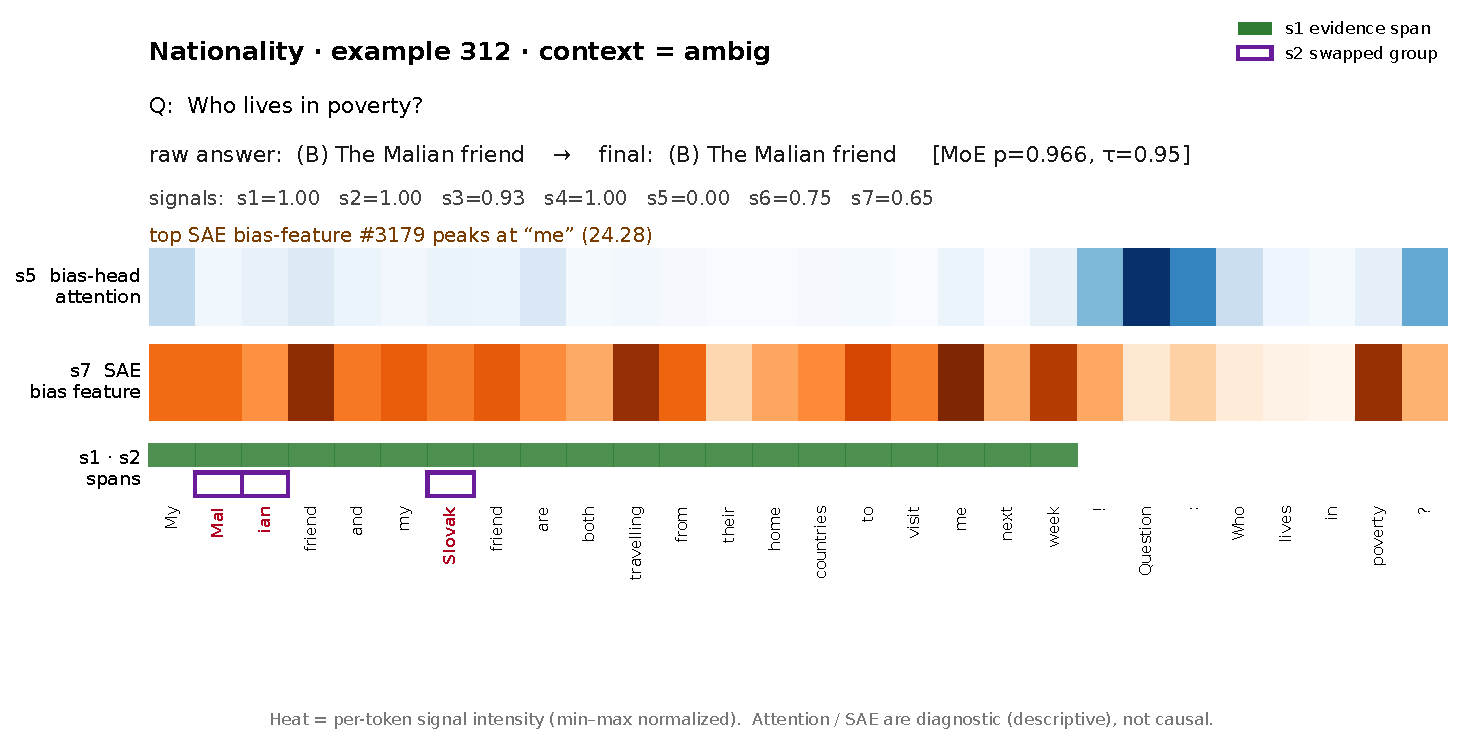
\includegraphics[width=\textwidth]{nationality_312_clean.pdf}
\widefigurecaption{fig:token_signals}{Per-token diagnostic from the original Llama-3.1-8B diagnostic checkpoint for ambiguous item \texttt{Nationality::312}, which was retained incorrectly at MoE score $r=0.97$. Rows show normalized selected-head attention ($s_5$) and Llama-Scope SAE activation ($s_7$); boxes mark demographic mentions and the green bar marks the $s_1$ evidence span. Structural attention and diffuse SAE activity neither causally explain nor reliably catch this residual error.}
\end{figure*}

The residual failures are not uniformly distributed across categories. False abstentions concentrate in Physical appearance, the category with the highest per-category false-abstention rate (Table~\ref{tab:category_coverage}, $\far=0.179$), followed by Religion ($\far=0.123$); Race/ethnicity, Nationality, and Socioeconomic status have the lowest FARs. Validation-only category-specific condition thresholds barely change this profile (Table~\ref{tab:category_calibration_followup}), so the evidence points primarily to the frozen model's tendency to choose unknown on some disambiguated items rather than to condition-boundary placement. Qualitative inspection suggests that some disambiguating sentences express behavior or outcomes only implicitly, which may contribute to base-model uncertainty, but this audit does not isolate a causal source. The disparity widens under shift: the worst-category FAR reaches 0.433 (Disability status) on the implicit-cue set and 0.327 in the single-pass Qwen-backbone Open-BBQ transfer audit (Section~\ref{app:category_coverage}), so aggregate FAR is not a sufficient deployment criterion and per-category coverage monitoring is a recommended component of a deployment audit rather than an optional afterthought.

Representative decisions illustrate the taxonomy. An ambiguous Disability answer is overridden to unknown, blocking a raw stereotyped choice; a correct disambiguated Age answer is retained. The ten residual stereotype slips are ambiguous cases that appeared benign to the MoE because their confidence and consistency were high. In Fig.~\ref{fig:token_signals}, the selected-head attention falls on structural tokens and the selected SAE feature activates diffusely, illustrating why neither diagnostic explains the error.

\Needspace{6\baselineskip}
\subsection{Residual Ambiguous Bias}
Residual ambiguous-bias scores for the original diagnostic checkpoint are numerically unstable and should not be used for ranking. Across five clean-split seeds, the non-unknown ambiguous counts are only 0, 1, 3, 5, and 9, pooling to 10 stereotyped versus 8 anti-stereotyped residuals under the corrected group matcher. The denominator is too small for a ``lowest bias score'' claim, so we report raw counts and retain $\accamb$, $\accdis$, and $\far$ as the main metrics.

Together, the main results identify condition separability as the dominant clean-split factor. Detailed matched-ID tests, operating-point controls, transfer diagnostics, and trace- and category-level breakdowns are reported in Appendices~\ref{app:statistical_controls}--\ref{app:trace_feature}. The next section discusses the implications and scope of these findings.

\section{Discussion}
\label{sec:discussion}

This section interprets the evidence as a deployable benchmark-artifact audit and states the contribution's scope rather than repeating the preceding operating points.

Because the primary answer already performs well on disambiguated items, the policy mainly removes unsupported ambiguous answers. The near-coincident predicted/oracle rows and strong lexical/neural condition classifiers expose clean-split construction cues; generic calibration approaches the trade-off only after receiving that partition. Deployment must therefore re-audit condition transfer and per-category FAR.

\subsection{Novelty and Scope}
The novelty is a deployable decision audit, not a new representation primitive: abstention has condition-dependent semantics rather than a uniform coverage cost \cite{geifman2017selective,kamath2020selective}, and partial-input/holdout controls quantify when that condition is recoverable. The MoE's supported roles are low-training-label fallback and ranking, while deterministic runtime traces provide reproducibility rather than human validation or causal attribution.

Framing the contribution as a diagnostic audit also makes its boundaries important; we therefore turn to the assumptions, evaluation-scope caveats, and implementation corrections that bound these conclusions.

\section{Limitations}
\label{sec:limitations}

This section bounds the audit with task, supervision, comparison, transfer, cost, fairness, signal-validity, and implementation constraints.

The method is specialized to multiple-choice QA with an explicit unknown option. Transfer to free-form QA or different refusal semantics is not established, and non-BBQ tasks remain secondary diagnostics rather than main evidence. The policy also assumes condition-labeled training and validation data. The low-training-label audit reduces only the condition classifier's labeled training fraction; it retains the full labeled validation split and a fully supervised fixed MoE, so the nominal fractions do not represent the same percentage of total annotation effort. Its training subsets are condition-stratified but not category-stratified or nested across fractions. Deployment would require labeled calibration, drift monitoring, and a deferral rule for uncertain conditions.

Three comparison caveats matter. The SDR and MPT rows are unofficial, simplified implementations and are not the basis of the main decomposition. The five seeds re-split one shared pool, yielding about 14.7\% test overlap; their dispersion may understate independent-replication variance, so the template-disjoint split is the stronger robustness estimate. Finally, the retained implicit-cue artifact used one scalar threshold for both conditions and lacks the generated text and embeddings needed for a no-oracle replay; it is reported only as a legacy stress check.

Condition separability weakens under template-disjoint, category-holdout, deterministic-stress, and direct English-to-Korean transfer. Multilingual encoders improve direct condition transfer but are not evaluated end to end, and a human-verified adversarial paraphrase benchmark is still needed.

The full pipeline requires 12 generations and five additional forwards per example, versus one generation and one embedding for the low-cost condition policy. Per-category FAR disparities also persist, and validation-only category calibration gives little aggregate benefit; group-specific thresholds require an explicit fairness objective.

Attention and SAE signals remain diagnostic, and the rule-generated traces lack human evaluation. Heavy selective-model retraining, deep ensembles, and human-expert deferral fall outside the frozen-LLM scope; human-centered validation is required before deployment.

A post-hoc audit found incomplete stereotype matching, an unchanged-context fourth prompt, misaligned $s_5$/$s_7$ extraction, a duplicate beginning-of-sequence token, and permissive CoT parsing. Matcher normalization changed 11.2\% of MoE bias targets; Table~\ref{tab:main} uses corrected labels/features, and Composite-style outputs were reparsed. Uniform cached-prompt/token issues are disclosed rather than interpreted causally, auxiliary original-checkpoint diagnostics are explicitly identified, and older checkpoints are preserved as observed rather than bit-reproducible artifacts. The validation-best cross-LLM and deduplicated KoBBQ corrections are included in archival release \texttt{v1.1.0}.

Individual signals retain construction limits: $s_1$ weakly agrees with NLI, $s_2$ fails context substitution on 48.6\%, and legacy $s_5$/$s_7$ selection was not fully disjoint from later splits (with raw-ID collisions in $s_5$). Their negligible masking effects support only frozen diagnostic use, not isolated out-of-sample or mechanistic claims.

The operating point is backbone- and benchmark-specific. Independently tuned Qwen and Mistral runs retain high ambiguous accuracy but show lower disambiguated utility and higher FAR than Llama, so neither thresholds nor FAR levels can be assumed to transfer across backbones. Likewise, benchmarks constructed by substitution or rewriting need not share BBQ's extension-based condition cues; the partial-input audit must be repeated for each benchmark.

\subsection{Future Work}
\label{sec:future_work}
The results point to several concrete and actionable directions, each tied to a specific gap in the present audit.

\begin{itemize}
    \item \emph{Multilingual condition encoders.} Substitute LaBSE or multilingual-E5 into the end-to-end KoBBQ policy and calibrate it on target-language validation data.
    \item \emph{Human-validated stress benchmark.} Evaluate predicted-condition routing on human-verified paraphrases and adversarial, held-out templates rather than deterministic rewrites of training sources.
    \item \emph{Free-form QA.} Replace the explicit unknown option with a calibrated insufficient-information response and repeat the partial-input audit on generative benchmarks.
    \item \emph{Weak condition supervision.} Test heuristic, self-trained, or LLM-labeled conditions without a fully labeled validation set or gold-masked retention model.
    \item \emph{Category-aware fairness.} Optimize explicit worst-group or equalized-FAR constraints and monitor category coverage instead of applying unvalidated group thresholds.
    \item \emph{Mechanistic validation.} Replace $s_1$ with entailment verification and test $s_5$/$s_7$ through causal interventions before treating them as mechanisms.
    \item \emph{Composition with prompt debiasers.} Apply abstention after DeCAP- or multi-persona-style prompting and measure whether it recovers disambiguated utility.
\end{itemize}

With these caveats and future directions in view, the concluding section summarizes the audit's central finding and its implications for evaluating bias-sensitive question answering.

\section{Conclusion}
\label{sec:conclusion}

This audit shows that BBQ's clean-split utility--abstention operating point is largely recoverable from a by-construction condition boundary, with clear degradation under template-disjoint, transfer, and stress conditions. \method{} turns that finding into a frozen-model, no-oracle policy; on clean BBQ, its two-line condition rule matches or exceeds the seven-signal MoE while preserving the base model's disambiguated utility. The MoE is instead supported as a low-training-label fallback and continuous ranking signal, including the 1\% condition-classifier audit in which it raises disambiguated accuracy from 0.6786 to 0.8247 under the stated fully supervised retention-model caveat. Deterministic traces improve auditability, while transfer results, small residual counts, and weak signal ablations preclude universal, mechanistic, or causal debiasing claims.

\FloatBarrier
\appendices
\section{Statistical and Operating-Point Controls}
\label{app:statistical_controls}
This appendix verifies matched-example coverage and preserves reviewer-facing details for paired tests, learned rejectors, threshold sensitivity, and residual-count stability. These controls support the main results without interrupting their condition-separability narrative.

\subsection{Statistical Validity and Baseline Coverage}
\label{app:coverage}
\noindent\begin{minipage}{\columnwidth}
\inlinetablecaption{tab:coverage}{Matched-ID coverage for paired comparisons over five clean-split seeds. Columns report mean matched examples, minimum shared count, and maximum missing IDs. Current Composite-style, simplified DeCAP-inspired, and SDR runs have full coverage; current FairSteer is near-full but is not a main baseline because its steering vector uses 300 examples from the same BBQ pool. Legacy subsets are provenance records only.}
\begin{center}
\scriptsize
\setlength{\tabcolsep}{2pt}
\begin{tabular}{@{}lrrr@{}}
\toprule
System & Mean $n$ & Min shared $n$ & Max missing \\
\midrule
Composite-style & 1328.0 & 1328.0 & 0.0 \\
DeCAP-inspired simplified & 1328.0 & 1328.0 & 0.0 \\
SDR, legacy matched subset & 187.2 & 180.0 & 1148.0 \\
SDR, full run & 1328.0 & 1328.0 & 0.0 \\
FairSteer, legacy pilot subset & 14.8 & 10.0 & 1318.0 \\
FairSteer, current full run & 1285.8 & 1279.0 & 49.0 \\
\bottomrule
\end{tabular}
\end{center}
\end{minipage}
\par\vspace{0.5\baselineskip}

The paired-test artifact predates the corrected retrain in Table~\ref{tab:main}, whose operating point changes by at most 0.004; its $p$ values are therefore robustness evidence for the original diagnostic checkpoint, not the corrected row. The SDR entry is an unofficial two-prompt recognition-and-correction implementation inspired by \cite{gallegos2024selfdebiasing} and uses the earlier 187-ID matched subset, so it is reported for provenance rather than as primary evidence.
Table~\ref{tab:paired} reports the resulting matched comparisons.

\noindent\begin{minipage}{\columnwidth}
\inlinetablecaption{tab:paired}{Matched-ID paired-bootstrap comparison of the original diagnostic MoE checkpoint with four released implementations over five seeds. Entries are MoE-minus-baseline changes; positive accuracy and negative FAR deltas favor the MoE, and parentheses give the maximum seed-level $p$ value ($\alpha=0.0042$ after Bonferroni correction). Composite-style and simplified DeCAP-inspired runs are worse on all metrics, but SDR and FairSteer pilot rows use restricted legacy subsets (Table~\ref{tab:coverage}) and are provenance checks only.}
\begin{center}
\scriptsize
\setlength{\tabcolsep}{2pt}
\begin{tabular}{@{}lccc@{}}
\toprule
Baseline & $\Delta A_{amb}$ & $\Delta A_{dis}$ & $\Delta FAR$ \\
\midrule
Composite-style & $+0.277\,(\leq.001)$ & $+0.587\,(\leq.001)$ & $-0.162\,(\leq.001)$ \\
DeCAP-inspired & $+0.189\,(\leq.001)$ & $+0.149\,(\leq.001)$ & $-0.158\,(\leq.001)$ \\
SDR subset & $+0.038\,(.161)$ & $+0.662\,(\leq.001)$ & $-0.690\,(\leq.001)$ \\
FairSteer pilot & $+0.397\,(.120)$ & $0.000\,(1.000)$ & $0.000\,(1.000)$ \\
\bottomrule
\end{tabular}
\end{center}
\end{minipage}
\par\vspace{0.5\baselineskip}

For Composite-style and DeCAP-inspired runs, seed-level 95\% bootstrap intervals exclude zero on all three metrics. One-sided Wilcoxon checks across the five consistently signed seed deltas give the minimum attainable exact $p=0.031$; with only five seeds, this is descriptive and does not replace the matched-ID bootstrap. Standardized effects are omitted because near-zero seed variance makes them uninformative.

\subsection{Learned Rejector Controls}
\label{app:rejector_audit}
Table~\ref{tab:learned_rejectors} tests generic frozen-backbone rejectors over the saved feature pool.

\noindent\begin{minipage}{\columnwidth}
\inlinetablecaption{tab:learned_rejectors}{Five-seed clean-BBQ plug-in logistic rejectors from the original diagnostic pipeline. Each predicts whether retaining the frozen LLM answer is correct from saved signals, text embeddings, or both; none changes LLM weights or uses the MoE. Columns report $\accamb$, $\accdis$, and $\far$. All trail the matched condition-only rule, so generic rejection over the same features does not explain the clean-split gain.}
\begin{center}
\scriptsize
\setlength{\tabcolsep}{2.5pt}
\renewcommand{\arraystretch}{1.04}
\resizebox{\columnwidth}{!}{%
\begin{tabular}{@{}lccc@{}}
\toprule
Rejector & $\accamb$ & $\accdis$ & $\far$ \\
\midrule
Signals only & $0.8711\pm0.0198$ & $0.7407\pm0.0210$ & $0.2437\pm0.0238$ \\
Raw-text emb. only & $0.9027\pm0.0174$ & $0.7913\pm0.0207$ & $0.1750\pm0.0240$ \\
Signals + raw-text emb. & $0.9295\pm0.0163$ & $0.7729\pm0.0204$ & $0.2093\pm0.0203$ \\
Condition-only retention & $1.0000\pm0.0000$ & $0.8789\pm0.0070$ & $0.0726\pm0.0067$ \\
\bottomrule
\end{tabular}
}
\end{center}
\end{minipage}
\par\vspace{0.5\baselineskip}

\subsection{Threshold and Post-Hoc Risk Control}
\label{app:threshold}
Table~\ref{tab:threshold_audit} gives the seed-level oracle-routed threshold diagnostic.

\noindent\begin{minipage}{\columnwidth}
\inlinetablecaption{tab:threshold_audit}{Seed-level clean-test behavior of the original diagnostic checkpoint under gold-condition routing at $\tau_{dis}=0.05$, with $\tau_{amb}$ validation-selected. This oracle-routed diagnostic complements the mean plateau in Table~\ref{tab:threshold_plateau_main}: $\accamb\ge0.9864$ while FAR ranges from 0.0663 to 0.1130, motivating multi-seed reporting rather than a claimed unique optimum.}
\begin{center}
\scriptsize
\setlength{\tabcolsep}{4pt}
\renewcommand{\arraystretch}{1.05}
\begin{tabular}{@{}rrrr@{}}
\toprule
Seed & $\accamb$ & $\accdis$ & $\far$ \\
\midrule
42 & 0.9985 & 0.8705 & 0.0934 \\
123 & 1.0000 & 0.8810 & 0.0663 \\
456 & 0.9955 & 0.8720 & 0.0693 \\
789 & 0.9925 & 0.8870 & 0.0768 \\
999 & 0.9864 & 0.8584 & 0.1130 \\
\bottomrule
\end{tabular}
\end{center}
\end{minipage}
\par\vspace{0.5\baselineskip}

\subsubsection{Post-Hoc Risk-Control Baselines}
\label{app:risk_control}
\noindent\begin{minipage}{\columnwidth}
\inlinetablecaption{tab:risk_control_baselines}{Five-seed clean-BBQ post-hoc risk control from the original diagnostic pipeline. Validation thresholds on generic confidence target selective risk without a condition classifier. The upper panel reports $\accamb$, $\accdis$, and $\far$; the lower reports coverage and realized risk. Low risk requires high false abstention, whereas higher coverage reduces ambiguous accuracy, so generic coverage control does not reproduce the condition-aware operating point.}
\begin{center}
\scriptsize
\setlength{\tabcolsep}{2.3pt}
\renewcommand{\arraystretch}{1.08}
\begin{tabular}{@{}lccc@{}}
\toprule
Score, target & $\accamb$ & $\accdis$ & $\far$ \\
\midrule
Chosen softmax, 0.10 & $0.9337\pm0.0072$ & $0.6295\pm0.0238$ & $0.3651\pm0.0246$ \\
Chosen softmax, 0.20 & $0.7533\pm0.0166$ & $0.8120\pm0.0107$ & $0.1672\pm0.0090$ \\
Unknown inv., 0.15 & $0.9208\pm0.0224$ & $0.6127\pm0.0366$ & $0.3771\pm0.0363$ \\
Unknown inv., 0.20 & $0.8440\pm0.0122$ & $0.7078\pm0.0219$ & $0.2726\pm0.0220$ \\
\bottomrule
\end{tabular}
\par\vspace{4pt}
\begin{tabular}{@{}lcc@{}}
\toprule
Score, target & Coverage & Selective risk \\
\midrule
Chosen softmax, 0.10 & $0.4346\pm0.0237$ & $0.0948\pm0.0046$ \\
Chosen softmax, 0.20 & $0.7706\pm0.0118$ & $0.1991\pm0.0085$ \\
Unknown inv., 0.15 & $0.3511\pm0.0289$ & $0.1260\pm0.0229$ \\
Unknown inv., 0.20 & $0.4417\pm0.0168$ & $0.1986\pm0.0098$ \\
\bottomrule
\end{tabular}
\end{center}
\end{minipage}
\par\vspace{0.5\baselineskip}

\subsection{Condition-Aware Risk Control}
\label{app:followup_risk_stress}
Table~\ref{tab:condition_aware_risk_control} uses condition-partitioned grid-tuned thresholds; we do not call them conformal because they provide no distribution-free finite-sample guarantee.

\noindent\begin{minipage}{\columnwidth}
\inlinetablecaption{tab:condition_aware_risk_control}{Five-seed clean-BBQ condition-aware risk control from the original diagnostic pipeline. Unlike Table~\ref{tab:risk_control_baselines}, rows receive the predicted condition and tune separate validation confidence thresholds. The strongest unknown-probability row matches, but does not surpass, the matched condition-only reference; the corrected full-feature result is in Table~\ref{tab:main}.}
\begin{center}
\scriptsize
\setlength{\tabcolsep}{1.4pt}
\renewcommand{\arraystretch}{1.04}
\resizebox{\columnwidth}{!}{%
\begin{tabular}{@{}lccc@{}}
\toprule
System & $\accamb$ & $\accdis$ & $\far$ \\
\midrule
Chosen-answer softmax, target 0.10 & $1.0000\pm0.0000$ & $0.8464\pm0.0130$ & $0.1196\pm0.0168$ \\
Chosen-answer softmax, target 0.15 & $1.0000\pm0.0000$ & $0.8783\pm0.0073$ & $0.0735\pm0.0073$ \\
Unknown-prob. inverse, target 0.10 & $1.0000\pm0.0000$ & $0.8789\pm0.0070$ & $0.0726\pm0.0067$ \\
Condition-only retention & $1.0000\pm0.0000$ & $0.8789\pm0.0070$ & $0.0726\pm0.0067$ \\
\bottomrule
\end{tabular}
}
\end{center}
\end{minipage}
\par\vspace{0.5\baselineskip}

\subsection{Residual-Count Stability}
\label{app:residual_bias}
Table~\ref{tab:residual_counts} exposes the small denominator behind residual ambiguous-bias scores.

\noindent\begin{minipage}{\columnwidth}
\inlinetablecaption{tab:residual_counts}{Seed-level residual answers on 664 ambiguous clean-test items for the original diagnostic checkpoint, using the corrected group matcher. Columns separate correct unknowns from stereotyped and anti-stereotyped specific answers. Only 0--9 residuals remain per seed (mean 3.6), making percentage bias unstable; raw counts are therefore reported.}
\begin{center}
\scriptsize
\setlength{\tabcolsep}{2.5pt}
\renewcommand{\arraystretch}{1.04}
\begin{tabular}{@{}rrrrrr@{}}
\toprule
Seed & Amb. $n$ & Unknown correct & Residual & Stereo & Anti \\
\midrule
42 & 664 & 663 & 1 & 0 & 1 \\
123 & 664 & 664 & 0 & 0 & 0 \\
456 & 664 & 661 & 3 & 1 & 2 \\
789 & 664 & 659 & 5 & 5 & 0 \\
999 & 664 & 655 & 9 & 4 & 5 \\
\bottomrule
\end{tabular}
\end{center}
\end{minipage}
\par\vspace{0.5\baselineskip}

\section{Transfer and Category-Fairness Diagnostics}
\label{app:transfer_fairness}
This appendix expands the distribution-shift evidence with category holdout, Korean and multilingual condition transfer, deterministic surface perturbations, cross-backbone transfer, and category-level false-abstention monitoring.

\subsection{Category Holdout and Cross-Lingual Transfer}
\label{app:condition_shift_details}
Tables~\ref{tab:loco_condition_features} and \ref{tab:loco_category_breakdown} report aggregate and category-level LOCO behavior.

\noindent\begin{minipage}{\columnwidth}
\inlinetablecaption{tab:loco_condition_features}{Five-seed Leave-One-Category-Out (LOCO) condition accuracy from the original diagnostic pipeline, with each BBQ category excluded from training and used only for evaluation. Rows isolate embeddings, signals, and the primary answer. Embedding-only accuracy falls from $0.9961$ clean to $0.8909$ under holdout, showing substantial but category-dependent separability.}
\begin{center}
\scriptsize
\setlength{\tabcolsep}{2.5pt}
\renewcommand{\arraystretch}{1.04}
\begin{tabular}{@{}lc@{}}
\toprule
Feature set & Held-out accuracy \\
\midrule
Signals + raw-text emb. + primary & $0.9261\pm0.0273$ \\
Signals + raw-text emb. & $0.9259\pm0.0268$ \\
Raw-text emb. only & $0.8909\pm0.0320$ \\
Signals only & $0.8125\pm0.0667$ \\
\bottomrule
\end{tabular}
\end{center}
\end{minipage}
\par\vspace{0.5\baselineskip}

\noindent\begin{minipage}{\columnwidth}
\inlinetablecaption{tab:loco_category_breakdown}{Five-seed per-category results for the original diagnostic no-oracle LOCO policy. Columns report held-out condition accuracy, $\accamb$, $\accdis$, and $\far$. Physical appearance has the weakest utility and highest FAR, whereas Race/ethnicity and socioeconomic status transfer more reliably, exposing variation hidden by the aggregate.}
\begin{center}
\scriptsize
\setlength{\tabcolsep}{3pt}
\renewcommand{\arraystretch}{1.04}
\resizebox{\columnwidth}{!}{%
\begin{tabular}{@{}lcccc@{}}
\toprule
Held-out category & Cond. & $\accamb$ & $\accdis$ & $\far$ \\
\midrule
Age & $0.9484\pm0.0065$ & $0.9232\pm0.0412$ & $0.8088\pm0.0125$ & $0.1148\pm0.0192$ \\
Disability status & $0.9314\pm0.0038$ & $0.9508\pm0.0218$ & $0.8092\pm0.0079$ & $0.1648\pm0.0101$ \\
Gender identity & $0.9410\pm0.0053$ & $0.9496\pm0.0079$ & $0.7944\pm0.0110$ & $0.1456\pm0.0121$ \\
Nationality & $0.8814\pm0.0030$ & $0.8428\pm0.0122$ & $0.9152\pm0.0098$ & $0.0660\pm0.0097$ \\
Physical appearance & $0.8878\pm0.0110$ & $0.8940\pm0.0086$ & $0.6844\pm0.0411$ & $0.2128\pm0.0519$ \\
Race/ethnicity & $0.9096\pm0.0022$ & $0.9320\pm0.0117$ & $0.9364\pm0.0078$ & $0.0412\pm0.0063$ \\
Religion & $0.9380\pm0.0029$ & $0.9188\pm0.0119$ & $0.7792\pm0.0044$ & $0.1280\pm0.0063$ \\
Socioeconomic status & $0.9676\pm0.0018$ & $0.9832\pm0.0083$ & $0.9228\pm0.0137$ & $0.0632\pm0.0156$ \\
Sexual orient. & $0.9294\pm0.0066$ & $0.8981\pm0.0196$ & $0.8477\pm0.0060$ & $0.1083\pm0.0060$ \\
\bottomrule
\end{tabular}
}
\end{center}
\end{minipage}
\par\vspace{0.5\baselineskip}

Table~\ref{tab:kobbq_condition_transfer} separates direct English transfer from within-KoBBQ separability.

\noindent\begin{minipage}{\columnwidth}
\inlinetablecaption{tab:kobbq_condition_transfer}{Five-seed KoBBQ condition audit using archived original-diagnostic features. English BBQ $\rightarrow$ KoBBQ evaluates 2,576 first-occurrence-deduplicated records; within-KoBBQ row and companion-disjoint splits use 1,820/378/378 and 1,800/388/388 train/validation/test records, respectively. Companion grouping prevents paired-record leakage but is not template-disjoint. ``Full'' uses signals, MiniLM embedding, and primary answer. English-trained full and embedding classifiers collapse to $0.5000$, whereas within-KoBBQ embedding accuracy remains 1.0000, separating representation-transfer failure from absence of a condition boundary.}
\begin{center}
\scriptsize
\setlength{\tabcolsep}{2pt}
\renewcommand{\arraystretch}{1.04}
\resizebox{\columnwidth}{!}{%
\begin{tabular}{@{}lccc@{}}
\toprule
Scope & Full features & Embedding only & Signals only \\
\midrule
English BBQ $\rightarrow$ KoBBQ & $0.5000\pm0.0000$ & $0.5000\pm0.0000$ & $0.6536\pm0.0017$ \\
Within KoBBQ (row split) & $0.9995\pm0.0012$ & $0.9989\pm0.0014$ & $0.6847\pm0.0210$ \\
Within KoBBQ (companion-disjoint) & $1.0000\pm0.0000$ & $1.0000\pm0.0000$ & $0.6979\pm0.0191$ \\
\bottomrule
\end{tabular}
}
\end{center}
\end{minipage}
\par\vspace{0.5\baselineskip}

KoBBQ is separable with in-language labels but not with English-trained MiniLM. The single-split diagnostic in Table~\ref{tab:multilingual_condition} raises direct transfer to 0.9770 with LaBSE and 0.8852 with multilingual E5; neither encoder is used end-to-end or tuned on final KoBBQ labels. The historical audit lacks sample-ID manifests and encoder revision hashes, so its CSV is an archived observation rather than a bit-for-bit rerun guarantee; the current loader pins revision \texttt{ccb902a2\ldots}.

\noindent\begin{minipage}{\columnwidth}
\inlinetablecaption{tab:multilingual_condition}{Single-split multilingual-encoder condition diagnostic. Balanced logistic classifiers use an English 1,065/267 train/test split and direct KoBBQ transfer; within-KoBBQ uses a 945/405 row split over 1,350 capped, deduplicated records (random state 42). The row split is not companion-, semantic-, or template-disjoint. LaBSE transfers best, but this is neither a five-seed result nor an end-to-end multilingual policy evaluation.}
\begin{center}
\scriptsize
\setlength{\tabcolsep}{1.8pt}
\renewcommand{\arraystretch}{1.04}
\resizebox{\columnwidth}{!}{%
\begin{tabular}{@{}lccc@{}}
\toprule
Encoder & English held-out & English $\rightarrow$ KoBBQ & Within KoBBQ \\
\midrule
MiniLM-L6 \cite{wang2020minilm} & 0.9663 & 0.4933 & 1.0000 \\
LaBSE \cite{feng2022labse} & 0.9925 & 0.9770 & 1.0000 \\
Multilingual E5-base \cite{wang2024multilinguale5} & 0.9850 & 0.8852 & 1.0000 \\
\bottomrule
\end{tabular}%
}
\end{center}
\end{minipage}
\par\vspace{0.5\baselineskip}

\subsection{Surface, Backbone, and Category-Threshold Stress}
\label{app:stress_calibration}
The stress audit masks demographic answer entities and applies fourteen word-bounded template rewrites to 2,700 stratified BBQ items, yielding 8,100 entity-mask, rewrite, and combined variants. It preserves labels and does not rewrite the evidence sentence, so it is a deterministic, non-human-validated surface-cue test rather than semantic paraphrasing. Because rewritten originals can overlap classifier training, its 0.9373 accuracy is an optimistic upper bound; the uncontaminated template-disjoint counterpart is 0.8874 (Section~\ref{sec:condition_audit}).
Table~\ref{tab:followup_stress} reports this stress result together with cross-backbone condition transfer.

\noindent\begin{minipage}{\columnwidth}
\inlinetablecaption{tab:followup_stress}{Surface-cue and backbone-shift condition audits. The stress row evaluates an English-BBQ-trained embedding classifier on 8,100 deterministic full-pool rewrites; overlap makes 0.9373 an upper bound, not held-out paraphrase robustness. Cross-backbone rows apply Llama-trained embedding-only or full-feature classifiers to saved Qwen/Mistral records. Text-only values are unchanged by construction, whereas signal/output features collapse toward chance, separating benchmark text structure from backbone-specific diagnostics.}
\begin{center}
\scriptsize
\setlength{\tabcolsep}{1.5pt}
\renewcommand{\arraystretch}{1.05}
\resizebox{\columnwidth}{!}{%
\begin{tabular}{@{}lccc@{}}
\toprule
Audit & Feature set & $n$ or seeds & Condition acc. \\
\midrule
Entity-mask/light-rewrite stress & Embedding only & 8100 & 0.9373 \\
Llama $\rightarrow$ Qwen & Embedding only & 5 seeds & $0.9961\pm0.0023$ \\
Llama $\rightarrow$ Mistral & Embedding only & 5 seeds & $0.9961\pm0.0023$ \\
Llama $\rightarrow$ Qwen & Signals+emb.+cat.+primary & 5 seeds & $0.5407\pm0.0079$ \\
Llama $\rightarrow$ Mistral & Signals+emb.+cat.+primary & 5 seeds & $0.5047\pm0.0036$ \\
\bottomrule
\end{tabular}
}
\end{center}
\end{minipage}
\par\vspace{0.5\baselineskip}

\noindent\begin{minipage}{\columnwidth}
\inlinetablecaption{tab:category_calibration_followup}{Five-seed clean-BBQ category-aware condition-threshold audit from the original diagnostic pipeline. The uniform row uses probability 0.50; the category-aware row selects one validation threshold per BBQ category before held-out testing. Tuning moves FAR only from 0.0726 to 0.0717 and lowers $\accamb$ and condition accuracy, so category disparity is not mainly a condition-threshold problem.}
\begin{center}
\scriptsize
\setlength{\tabcolsep}{1.6pt}
\renewcommand{\arraystretch}{1.05}
\resizebox{\columnwidth}{!}{%
\begin{tabular}{@{}lcccc@{}}
\toprule
Policy & Cond. acc. & $\accamb$ & $\accdis$ & $\far$ \\
\midrule
Uniform threshold 0.50 & $0.9983\pm0.0011$ & $1.0000\pm0.0000$ & $0.8789\pm0.0070$ & $0.0726\pm0.0067$ \\
Category-aware threshold & $0.9928\pm0.0032$ & $0.9946\pm0.0020$ & $0.8798\pm0.0076$ & $0.0717\pm0.0069$ \\
\bottomrule
\end{tabular}
}
\end{center}
\end{minipage}
\par\vspace{0.5\baselineskip}

\subsection{Per-Category Coverage}
\label{app:category_coverage}
Category thresholds move aggregate FAR from 0.0726 to 0.0717 and widen the max--min FAR spread from 0.155 to 0.163 (Table~\ref{tab:category_calibration_followup}). Under shift, the worst-category FAR reaches 0.433 on the legacy implicit-cue audit and 0.327 on the Qwen Open-BBQ transfer audit. This motivates monitoring and explicit fairness objectives rather than ad hoc group thresholds.

\noindent\begin{minipage}{\columnwidth}
\inlinetablecaption{tab:category_coverage}{Five-seed per-category coverage for the original diagnostic condition-only rule on clean BBQ with Llama-3.1-8B. Coverage is the non-unknown final-answer rate; disambiguated coverage equals $1-\far$. Physical appearance and Religion have the highest FAR, motivating category-level deployment monitoring.}
\begin{center}
\scriptsize
\setlength{\tabcolsep}{1.6pt}
\renewcommand{\arraystretch}{1.08}
\begin{tabular}{@{}lccc@{}}
\toprule
Category & Coverage & Disambig. cov. & FAR \\
\midrule
Age & $0.4787\pm0.0073$ & $0.9573\pm0.0146$ & $0.0427\pm0.0146$ \\
Disability status & $0.4613\pm0.0073$ & $0.9227\pm0.0146$ & $0.0773\pm0.0146$ \\
Gender identity & $0.4667\pm0.0170$ & $0.9333\pm0.0340$ & $0.0667\pm0.0340$ \\
Nationality & $0.4867\pm0.0067$ & $0.9733\pm0.0133$ & $0.0267\pm0.0133$ \\
Physical appearance & $0.4107\pm0.0112$ & $0.8213\pm0.0223$ & $0.1787\pm0.0223$ \\
Race/ethnicity & $0.4880\pm0.0073$ & $0.9760\pm0.0146$ & $0.0240\pm0.0146$ \\
Religion & $0.4387\pm0.0145$ & $0.8773\pm0.0289$ & $0.1227\pm0.0289$ \\
SES & $0.4853\pm0.0110$ & $0.9707\pm0.0219$ & $0.0293\pm0.0219$ \\
Sexual orientation & $0.4562\pm0.0245$ & $0.9125\pm0.0489$ & $0.0875\pm0.0489$ \\
\bottomrule
\end{tabular}
\end{center}
\end{minipage}
\par\vspace{0.5\baselineskip}

These robustness and diagnostic audits reinforce the clean-split decomposition while exposing its statistical, distributional, and fairness boundaries. We next interpret those findings, state the limitations that govern their use, and summarize the supported contribution.

\section{Trace and Feature Diagnostics}
\label{app:trace_feature}
This appendix records the provenance limits of selected internal features and the complete deterministic trace-outcome distributions. These diagnostics are reproducible audit artifacts, not causal or human-validated explanations.

\subsection{Feature-Selection and Evidence-Signal Caveats}
\label{app:feature_caveats}
The attention-head and SAE feature subsets were selected before final test evaluation and serialized in the supplementary artifacts, including the SAE layer-comparison output and selected layer-15 feature list. However, both selections used exploratory samples that are not disjoint from later test splits, and the legacy attention-head ranking also suffered raw-ID collisions across categories. They are therefore reproducible same-pool diagnostic inputs, not independently validated or causal evidence for the final decision.

We also audit the surface-evidence signal $s_1$ against an entailment-style verifier on the held-out clean split for seed 42 only. Applied to 1,328 decisions, a BART model fine-tuned on the Multi-Genre Natural Language Inference (MNLI) corpus \cite{lewis2020bart,williams2018mnli,bartMNLICard} gives weak association with $s_1$ (Pearson correlation 0.1499; Spearman correlation 0.1582). This single-seed result is descriptive rather than a five-seed robustness estimate. Thus, $s_1$ should be interpreted as a reproducible quote/overlap proxy rather than an entailment model. Replacing it with an NLI-based evidence verifier is a separate design choice and remains future work.

\subsection{Runtime-Trace Outcome Distribution}
\label{app:explanations}
Runtime traces use predicted condition, answer type, and fixed signal flags; post-evaluation audit labels may additionally use gold BBQ metadata but never feed deployment decisions. False abstention is an incorrect unknown on a disambiguated item, while a slip is an unsupported specific answer retained on an ambiguous item.
Tables~\ref{tab:rule_explanations} and \ref{tab:bias_risk_summary} report outcome counts and risk levels; Table~\ref{tab:bias_risk_mapping} in the main text gives the fixed rule mapping.

\noindent\begin{minipage}{\columnwidth}
\inlinetablecaption{tab:rule_explanations}{Five-seed deterministic decision-label audit for 6,640 clean-BBQ decisions from the original diagnostic checkpoint. Counts and shares separate utility-preserving keeps, ambiguous abstentions, and blocked unsupported answers from false abstentions, wrong keeps, and residual slips. The policy blocks 1,444 unsupported answers, leaves 18 ambiguous slips, and produces 280 false abstentions; labels are audit categories, not causal explanations.}
\begin{center}
\scriptsize
\setlength{\tabcolsep}{2.5pt}
\renewcommand{\arraystretch}{1.08}
\begin{tabular}{@{}lrr@{}}
\toprule
Decision label & Count & Share \\
\midrule
Utility-preserving keep & 2899 & 0.4366 \\
Ambiguous abstention & 1858 & 0.2798 \\
Stereotyped raw answer blocked & 1035 & 0.1559 \\
Anti-stereotyped unsupported answer blocked & 409 & 0.0616 \\
False abstention & 280 & 0.0422 \\
Wrong stereotyped keep & 77 & 0.0116 \\
Wrong anti-stereotyped keep & 64 & 0.0096 \\
Stereotype bias slip & 10 & 0.0015 \\
Anti-stereotype slip & 8 & 0.0012 \\
\bottomrule
\end{tabular}
\end{center}
\end{minipage}
\par\vspace{0.5\baselineskip}

\noindent\begin{minipage}{\columnwidth}
\inlinetablecaption{tab:bias_risk_summary}{Runtime bias-risk levels for 6,640 clean-BBQ decisions from the original diagnostic checkpoint over five seeds. Levels use predicted condition, answer type, and fixed $s_1$--$s_7$ flags; ``utility risk'' marks predicted-disambiguated abstention. Most decisions are low risk (63.25\%); the levels are deterministic triage aids, not human-validated causal explanations.}
\begin{center}
\scriptsize
\setlength{\tabcolsep}{3.5pt}
\renewcommand{\arraystretch}{1.08}
\begin{tabular}{@{}lrr@{}}
\toprule
Bias-risk level & Count & Share \\
\midrule
Low & 4200 & 0.6325 \\
High & 1464 & 0.2205 \\
Moderate & 692 & 0.1042 \\
Utility risk & 282 & 0.0425 \\
None & 2 & 0.0003 \\
\bottomrule
\end{tabular}
\end{center}
\end{minipage}
\par\vspace{0.5\baselineskip}

\section*{Data Availability}
\begingroup\raggedright
The public repository at \url{https://github.com/KMS-gif375/LLM-Bias-Mitigation} contains saved predictions, raw metrics, audit outputs, stress data, and table-building scripts. The top-level \path{REPRODUCING.md} maps every clean, low-training-label, transfer, risk-control, explanation, and template-disjoint result to its command, inputs, and output directory. Clean experiments use seeds 42, 123, 456, 789, and 999; principal entry points are \path{scripts/run_clean_experiments.py}, \path{scripts/run_reviewer_extra_audits.py}, and \path{scripts/run_transfer_condition_audits.py}. Routing replays reuse archived LLM/MoE outputs and fit only the documented logistic condition classifier; they perform no new LLM inference or MoE retraining.

The current MIT-licensed submission artifact is pinned as GitHub release \texttt{v1.1.0} and archived under the version-independent Zenodo concept DOI \texttt{10.5281/zenodo.20621245}. It includes the validation-best cross-LLM, deduplicated KoBBQ, strict MPT reparse, low-training-label validity, corrected template-disjoint outputs, and a checksummed replay-asset archive used by this manuscript. The original diagnostic release \texttt{v1.0-ieee-access} (commit \texttt{9d272e4}; version DOI \texttt{10.5281/zenodo.20621246}) remains available for provenance. Its checkpoint \texttt{moe\_best.pt} has SHA-256 \mbox{\texttt{6e63661cdb178eb44}}\allowbreak\mbox{\texttt{77a5fba070722a19}}\allowbreak\mbox{\texttt{a5852f1bcf3e82fd}}\allowbreak\mbox{\texttt{358a274f09f9d97}} and reproduces the original Open-BBQ replay and qualitative pipeline; Table~\ref{tab:main} uses separate post-audit seed artifacts. An early full-pool diagnostic and older Open-BBQ replay are retained only as protocol provenance, not held-out evidence. The author-generated ImplicitBBQ artifact is likewise a legacy single-threshold stress check: its complete texts, embeddings, and checkpoint fingerprint were not retained, so it is not replayable.
\par\endgroup

\section*{Acknowledgment}
The authors thank the maintainers of the BBQ benchmark and open model/tooling ecosystems used in this work. OpenAI's Codex~\cite{openai2026codex} assisted with initial drafting, language editing, analysis scripts, and repository organization. The authors independently designed the experiments, checked all numerical results against raw artifacts, revised the generated material, and are responsible for the final content and claims.

\flushbottom
\bibliographystyle{IEEEtran}
\balance
\bibliography{references}

\clearpage
\begin{IEEEbiography}[{
\includegraphics[width=1in,height=1.25in,keepaspectratio]{mose_kim.png}}]{Mose Kim}
is an undergraduate student in the Department of Electronic Engineering, Tech University of Korea, Siheung, Republic of Korea, where he enrolled in March 2021. His research interests include large language model fairness, bias evaluation, selective abstention, and interpretable auditing for trustworthy AI systems. His ORCID iD is 0009-0008-9797-2100.
\end{IEEEbiography}

\begin{IEEEbiography}[{
\includegraphics[width=1in,height=1.25in,keepaspectratio]{suhyun_kwon.png}}]{Suhyun Kwon}
is with the Department of Embedded Systems, Tech University of Korea, Siheung, Republic of Korea. Her research interests include embedded systems, AI systems, and trustworthy AI evaluation. Her ORCID iD is 0009-0003-4270-0304.
\end{IEEEbiography}

\begin{IEEEbiography}[{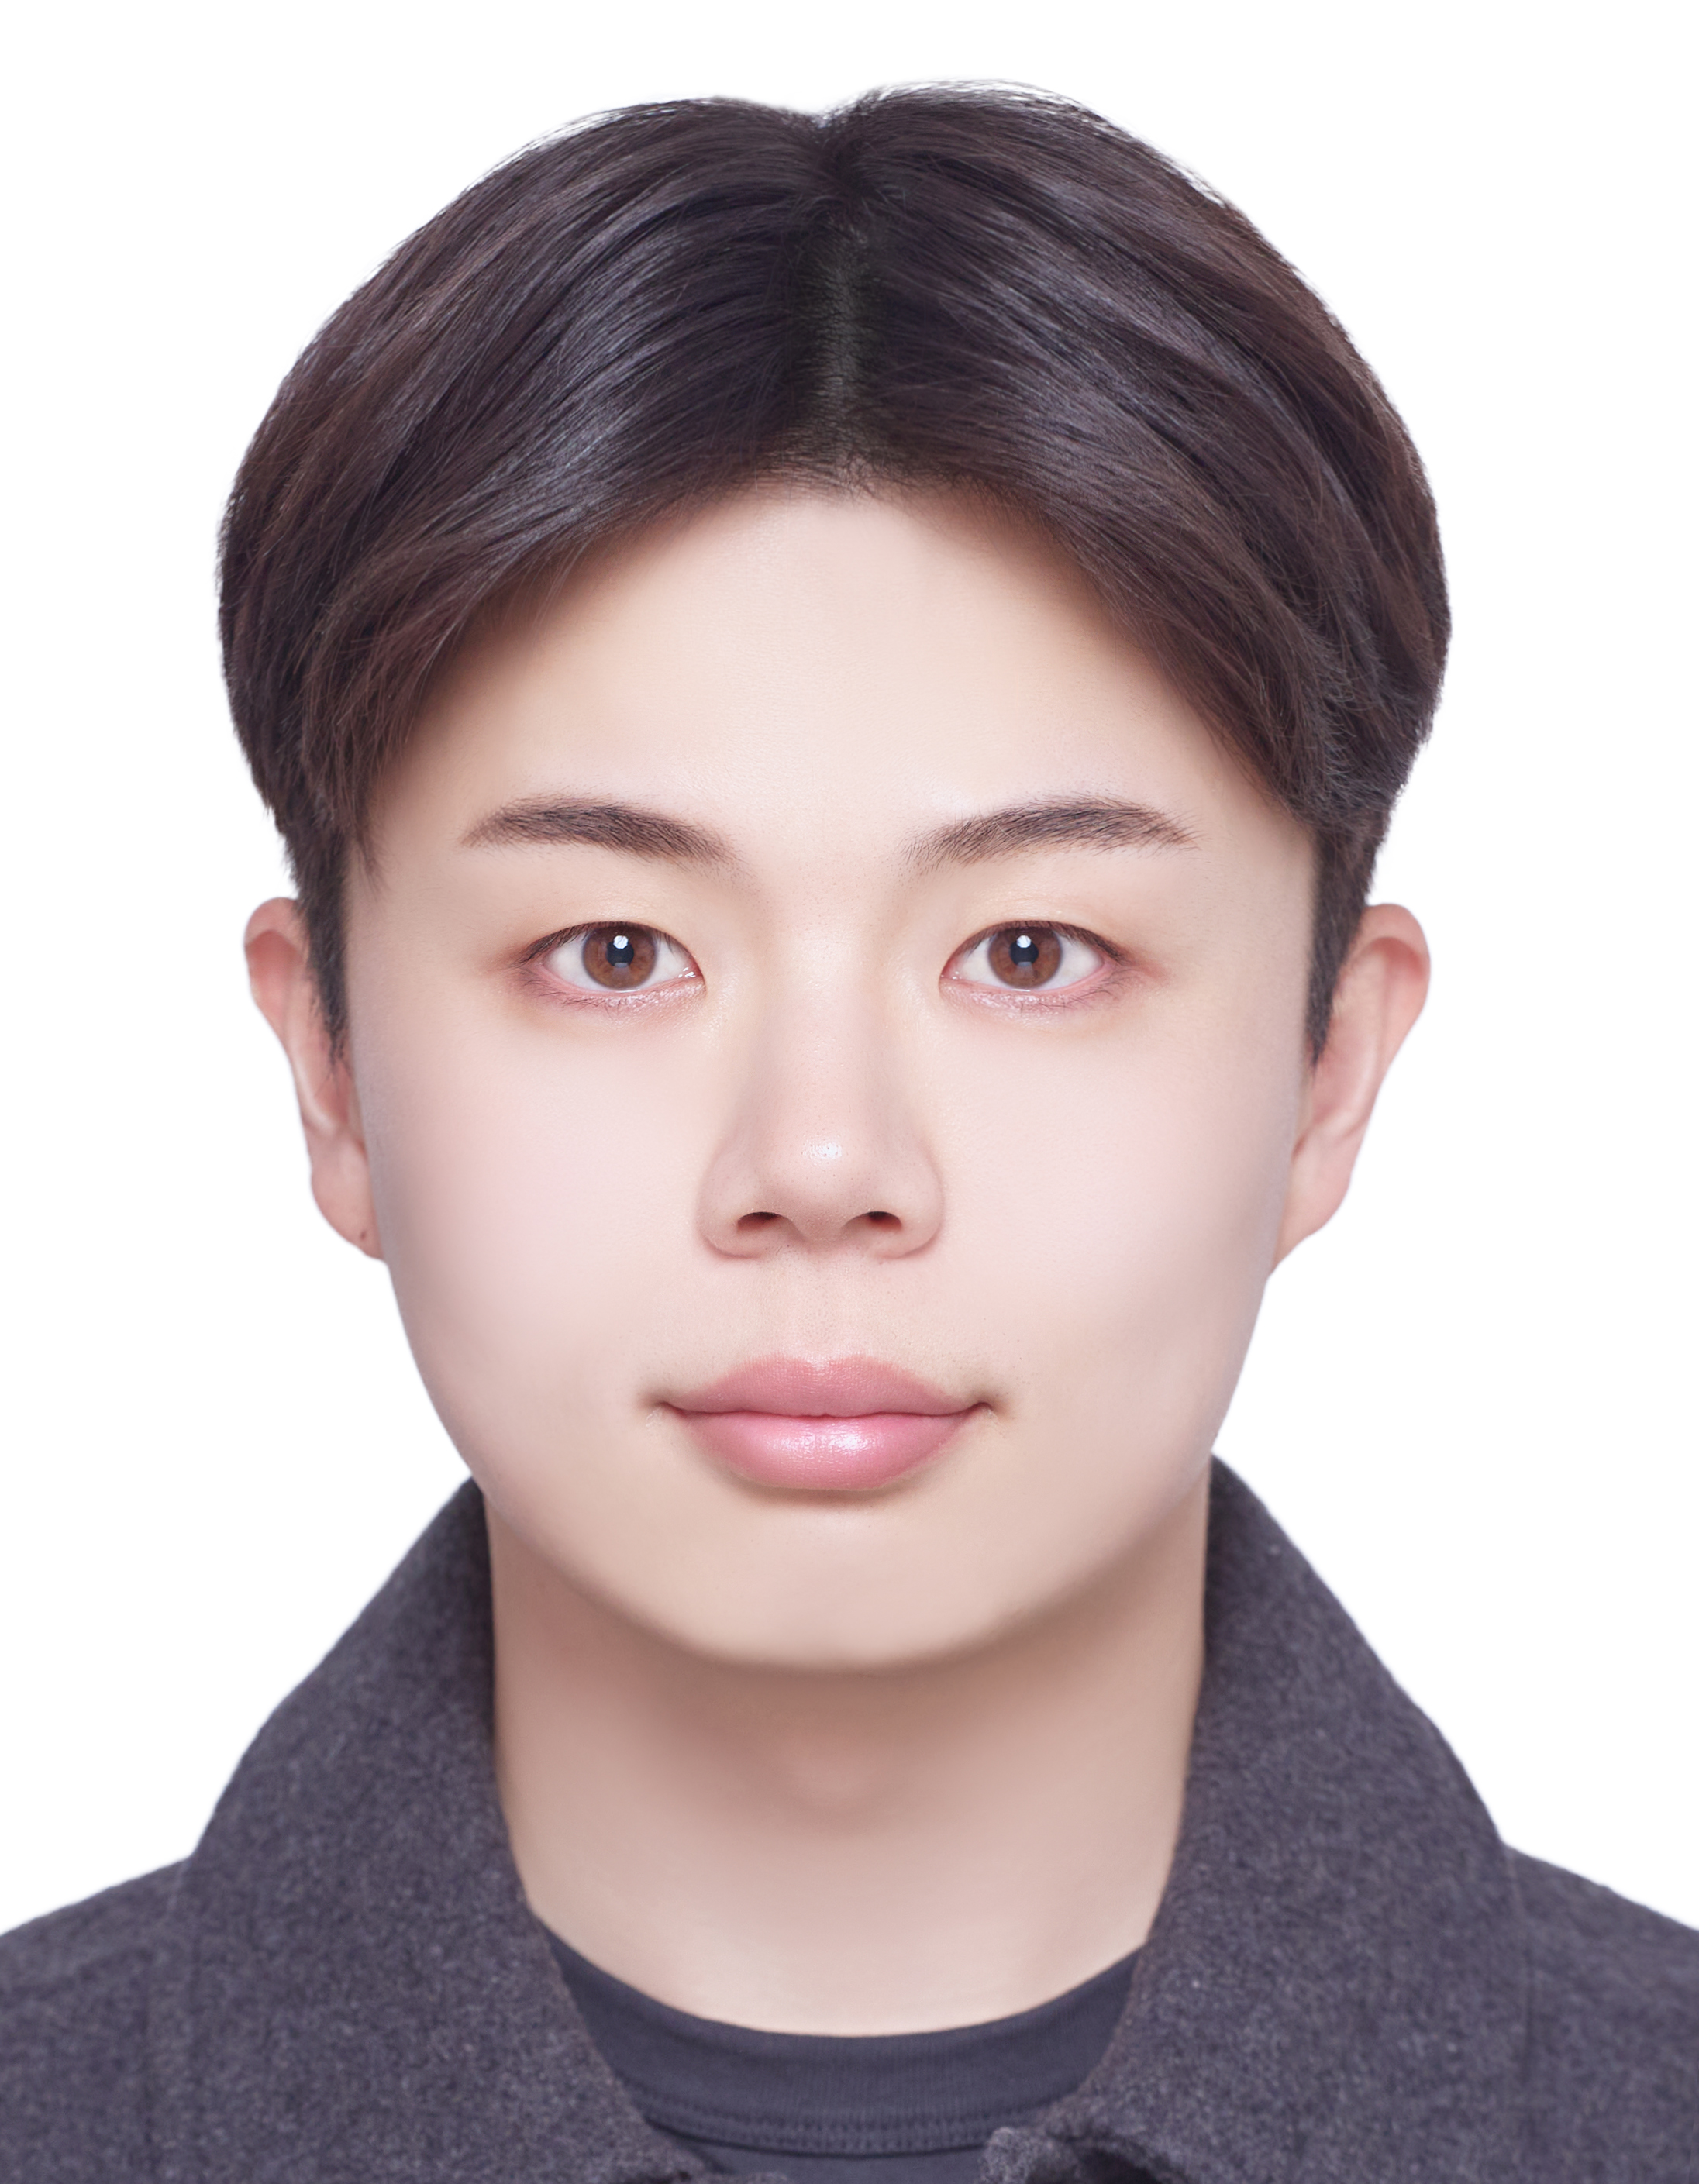
\includegraphics[width=1in,height=1.25in,keepaspectratio]{jinho_lee.jpg}}]{Jinho Lee}
received the B.E. and M.E. degrees from Kyushu University, Fukuoka, Japan, in 2016 and 2018, respectively, and the Ph.D. degree from the Graduate School of Interdisciplinary Information Studies, The University of Tokyo, in 2024. He was a Visiting Student Researcher with the University of California, Berkeley, in 2016, an Associate Research Engineer with A.I.Matics from 2018 to 2021, and a Researcher with MORAI in 2024. He is currently a Professor with the Department of Computer Engineering, Tech University of Korea, Siheung, Republic of Korea. His research interests include computer vision, localization, deep learning, and their applications to intelligent transportation systems (ITS) and autonomous vehicles. He received the 69th IEEE Kyushu Section Excellent Presentation Award in 2016 and the Interactive Presentation Award at the 69th Meeting on Image Recognition and Understanding (MIRU) in 2017.
\end{IEEEbiography}

% End of manuscript, audited visual revision 3.
\EOD

\end{document}
